\documentclass[orivec, envcountsame]{llncs}
\pagestyle{plain}

\usepackage[english]{babel}
\usepackage[modulo]{lineno}
\linenumbers

\usepackage{amssymb, amsmath}
\usepackage[backend=biber]{biblatex}
\usepackage{csquotes}
\addbibresource{phd.bib}
\usepackage{graphicx}
\usepackage[colorlinks=true, allcolors=blue]{hyperref}

\usepackage{tikz}
\usetikzlibrary{automata, positioning, arrows.meta}
 \newcommand{\eq}{=} % for automaton initial state
 
\usepackage{isabelle}
\usepackage{isabellesym}

\usepackage{ifthen}
\usepackage{bbold}

\usepackage{hyperref}

\newcommand{\isalogo}{\includegraphics[width=9pt]{./images/isabelle_transparent.png}}
\newcommand{\isalink}[1]{\href{#1}{\isalogo}}

\newcommand{\DefineSnippet}[2]{%
\expandafter\newcommand\csname snippet--#1\endcsname{%
 \begin{quote}
 \begin{isabelle}
 #2
 \end{isabelle}
 \end{quote}}}
\newcommand{\Snippet}[1]{%
\ifcsname snippet--#1\endcsname{\csname snippet--#1\endcsname}%
\else+++++++ERROR: Snippet ``#1 not defined+++++++ \fi}

\DefineSnippet{Wiener_kernel}{
\isacommand{definition}\isamarkupfalse%
\ Wiener{\isacharunderscore}{\kern0pt}kernel\ {\isacharcolon}{\kern0pt}{\isacharcolon}{\kern0pt}\ {\isachardoublequoteopen}real\ {\isasymRightarrow}\ real\ hkernel{\isachardoublequoteclose}\ \isakeyword{where}\isanewline
{\isachardoublequoteopen}Wiener{\isacharunderscore}{\kern0pt}kernel\ i\ {\isasymequiv}\ if\ i\ {\isacharequal}{\kern0pt}\ {\isadigit{0}}\ then\ hkernel\ {\isacharparenleft}{\kern0pt}return{\isacharunderscore}{\kern0pt}kernel\ borel{\isacharparenright}{\kern0pt}\isanewline
\ \ \ else\ hkernel{\isacharunderscore}{\kern0pt}of\ borel\ {\isacharparenleft}{\kern0pt}{\isasymlambda}x\ dy{\isachardot}{\kern0pt}\ {\isacharparenleft}{\kern0pt}return\ borel\ x\ {\isasymstar}\ density\ lborel\ {\isacharparenleft}{\kern0pt}normal{\isacharunderscore}{\kern0pt}density\ {\isadigit{0}}\ i{\isacharparenright}{\kern0pt}{\isacharparenright}{\kern0pt}\ dy{\isacharparenright}{\kern0pt}{\isachardoublequoteclose}%
}%EndSnippet
\DefineSnippet{brownian_motion}{
\isacommand{locale}\isamarkupfalse%
\ brownian{\isacharunderscore}{\kern0pt}motion\ {\isacharequal}{\kern0pt}\isanewline
\ \ \isakeyword{fixes}\ W\ {\isacharcolon}{\kern0pt}{\isacharcolon}{\kern0pt}\ {\isachardoublequoteopen}{\isacharparenleft}{\kern0pt}real{\isacharcomma}{\kern0pt}\ {\isacharprime}{\kern0pt}a{\isacharcomma}{\kern0pt}\ real{\isacharparenright}{\kern0pt}\ stochastic{\isacharunderscore}{\kern0pt}process{\isachardoublequoteclose}\isanewline
\ \ \isakeyword{assumes}\ init{\isacharunderscore}{\kern0pt}{\isadigit{0}}{\isacharbrackleft}{\kern0pt}simp{\isacharbrackright}{\kern0pt}{\isacharcolon}{\kern0pt}\ {\isachardoublequoteopen}W\ {\isadigit{0}}\ x\ {\isacharequal}{\kern0pt}\ {\isadigit{0}}{\isachardoublequoteclose}\ \isanewline
\ \ \ \ \ \ \isakeyword{and}\ source{\isacharcolon}{\kern0pt}\ {\isachardoublequoteopen}proc{\isacharunderscore}{\kern0pt}target\ W\ {\isacharequal}{\kern0pt}\ borel{\isachardoublequoteclose}\isanewline
\ \ \ \ \ \ \isakeyword{and}\ indep{\isacharunderscore}{\kern0pt}increments{\isacharcolon}{\kern0pt}\ {\isachardoublequoteopen}indep{\isacharunderscore}{\kern0pt}increments\ W{\isachardoublequoteclose}\isanewline
\ \ \ \ \ \ \isakeyword{and}\ normal{\isacharunderscore}{\kern0pt}increments{\isacharcolon}{\kern0pt}\ {\isachardoublequoteopen}{\isasymAnd}s\ t{\isachardot}{\kern0pt}\ {\isadigit{0}}\ {\isasymle}\ s\ {\isasymand}\ s\ {\isacharless}{\kern0pt}\ t\ {\isasymLongrightarrow}\isanewline
\ \ \ distributed\ M\ borel\ {\isacharparenleft}{\kern0pt}{\isasymlambda}v{\isachardot}{\kern0pt}\ W\ t\ v\ {\isacharminus}{\kern0pt}\ W\ s\ v{\isacharparenright}{\kern0pt}\ {\isacharparenleft}{\kern0pt}normal{\isacharunderscore}{\kern0pt}density\ {\isadigit{0}}\ {\isacharparenleft}{\kern0pt}sqrt\ {\isacharparenleft}{\kern0pt}t{\isacharminus}{\kern0pt}s{\isacharparenright}{\kern0pt}{\isacharparenright}{\kern0pt}{\isacharparenright}{\kern0pt}{\isachardoublequoteclose}%
}%EndSnippet
\DefineSnippet{kernel_product}{
\isacommand{definition}\isamarkupfalse%
\ kernel{\isacharunderscore}{\kern0pt}product\ {\isacharcolon}{\kern0pt}{\isacharcolon}{\kern0pt}\ {\isachardoublequoteopen}{\isacharparenleft}{\kern0pt}{\isacharprime}{\kern0pt}a{\isacharcomma}{\kern0pt}\ {\isacharprime}{\kern0pt}b{\isacharparenright}{\kern0pt}\ kernel\ {\isasymRightarrow}\ {\isacharparenleft}{\kern0pt}{\isacharprime}{\kern0pt}a\ {\isasymtimes}\ {\isacharprime}{\kern0pt}b{\isacharcomma}{\kern0pt}\ {\isacharprime}{\kern0pt}c{\isacharparenright}{\kern0pt}\ kernel\ {\isasymRightarrow}\ {\isacharparenleft}{\kern0pt}{\isacharprime}{\kern0pt}a{\isacharcomma}{\kern0pt}\ {\isacharprime}{\kern0pt}b\ {\isasymtimes}\ {\isacharprime}{\kern0pt}c{\isacharparenright}{\kern0pt}\ kernel{\isachardoublequoteclose}\ {\isacharparenleft}{\kern0pt}\isakeyword{infixr}\ {\isachardoublequoteopen}{\isacharparenleft}{\kern0pt}{\isasymOtimes}\isactrlsub K{\isacharparenright}{\kern0pt}{\isachardoublequoteclose}\ {\isadigit{9}}{\isadigit{0}}{\isacharparenright}{\kern0pt}\ \isakeyword{where}\isanewline
{\isachardoublequoteopen}kernel{\isacharunderscore}{\kern0pt}product\ K{\isacharunderscore}{\kern0pt}{\isadigit{1}}\ K{\isacharunderscore}{\kern0pt}{\isadigit{2}}\ {\isasymequiv}\ kernel{\isacharunderscore}{\kern0pt}of\ {\isacharparenleft}{\kern0pt}kernel{\isacharunderscore}{\kern0pt}source\ K{\isacharunderscore}{\kern0pt}{\isadigit{1}}{\isacharparenright}{\kern0pt}\ {\isacharparenleft}{\kern0pt}kernel{\isacharunderscore}{\kern0pt}target\ K{\isacharunderscore}{\kern0pt}{\isadigit{1}}\ {\isasymOtimes}\isactrlsub M\ kernel{\isacharunderscore}{\kern0pt}target\ K{\isacharunderscore}{\kern0pt}{\isadigit{2}}{\isacharparenright}{\kern0pt}\isanewline
\ \ {\isacharparenleft}{\kern0pt}{\isasymlambda}{\isasymomega}\isactrlsub {\isadigit{0}}\ A{\isachardot}{\kern0pt}\ {\isasymintegral}\isactrlsup {\isacharplus}{\kern0pt}{\isasymomega}\isactrlsub {\isadigit{1}}{\isachardot}{\kern0pt}\ {\isacharparenleft}{\kern0pt}{\isasymintegral}\isactrlsup {\isacharplus}{\kern0pt}{\isasymomega}\isactrlsub {\isadigit{2}}{\isachardot}{\kern0pt}\ indicator\ A\ {\isacharparenleft}{\kern0pt}{\isasymomega}\isactrlsub {\isadigit{1}}{\isacharcomma}{\kern0pt}\ {\isasymomega}\isactrlsub {\isadigit{2}}{\isacharparenright}{\kern0pt}{\isasympartial}kernel{\isacharunderscore}{\kern0pt}measure\ K{\isacharunderscore}{\kern0pt}{\isadigit{2}}\ {\isacharparenleft}{\kern0pt}{\isasymomega}\isactrlsub {\isadigit{0}}{\isacharcomma}{\kern0pt}\ {\isasymomega}\isactrlsub {\isadigit{1}}{\isacharparenright}{\kern0pt}{\isacharparenright}{\kern0pt}{\isasympartial}kernel{\isacharunderscore}{\kern0pt}measure\ K{\isacharunderscore}{\kern0pt}{\isadigit{1}}\ {\isasymomega}\isactrlsub {\isadigit{0}}{\isacharparenright}{\kern0pt}{\isachardoublequoteclose}%
}%EndSnippet
\DefineSnippet{kernel_product_partial}{
\isacommand{definition}\isamarkupfalse%
\ kernel{\isacharunderscore}{\kern0pt}product{\isacharunderscore}{\kern0pt}partial\ {\isacharcolon}{\kern0pt}{\isacharcolon}{\kern0pt}\ {\isachardoublequoteopen}{\isacharparenleft}{\kern0pt}{\isacharprime}{\kern0pt}a{\isacharcomma}{\kern0pt}\ {\isacharprime}{\kern0pt}b{\isacharparenright}{\kern0pt}\ kernel\ {\isasymRightarrow}\ {\isacharparenleft}{\kern0pt}{\isacharprime}{\kern0pt}b{\isacharcomma}{\kern0pt}\ {\isacharprime}{\kern0pt}c{\isacharparenright}{\kern0pt}\ kernel\ {\isasymRightarrow}\ {\isacharparenleft}{\kern0pt}{\isacharprime}{\kern0pt}a{\isacharcomma}{\kern0pt}\ {\isacharprime}{\kern0pt}b\ {\isasymtimes}\ {\isacharprime}{\kern0pt}c{\isacharparenright}{\kern0pt}\ kernel{\isachardoublequoteclose}\ {\isacharparenleft}{\kern0pt}\isakeyword{infixr}\ {\isachardoublequoteopen}{\isacharparenleft}{\kern0pt}{\isasymOtimes}\isactrlsub P{\isacharparenright}{\kern0pt}{\isachardoublequoteclose}\ {\isadigit{9}}{\isadigit{0}}{\isacharparenright}{\kern0pt}\ \isakeyword{where}\isanewline
{\isachardoublequoteopen}kernel{\isacharunderscore}{\kern0pt}product{\isacharunderscore}{\kern0pt}partial\ K{\isacharunderscore}{\kern0pt}{\isadigit{1}}\ K{\isacharunderscore}{\kern0pt}{\isadigit{2}}\ {\isasymequiv}\ K{\isacharunderscore}{\kern0pt}{\isadigit{1}}\ {\isasymOtimes}\isactrlsub K\ {\isacharparenleft}{\kern0pt}kernel{\isacharunderscore}{\kern0pt}of\ {\isacharparenleft}{\kern0pt}kernel{\isacharunderscore}{\kern0pt}source\ K{\isacharunderscore}{\kern0pt}{\isadigit{1}}\ {\isasymOtimes}\isactrlsub M\ kernel{\isacharunderscore}{\kern0pt}source\ K{\isacharunderscore}{\kern0pt}{\isadigit{2}}{\isacharparenright}{\kern0pt}\ {\isacharparenleft}{\kern0pt}kernel{\isacharunderscore}{\kern0pt}target\ K{\isacharunderscore}{\kern0pt}{\isadigit{2}}{\isacharparenright}{\kern0pt}\isanewline
\ {\isacharparenleft}{\kern0pt}{\isasymlambda}{\isasymomega}\ A\isactrlsub {\isadigit{2}}{\isachardot}{\kern0pt}\ kernel\ K{\isacharunderscore}{\kern0pt}{\isadigit{2}}\ {\isacharparenleft}{\kern0pt}snd\ {\isasymomega}{\isacharparenright}{\kern0pt}\ A\isactrlsub {\isadigit{2}}{\isacharparenright}{\kern0pt}{\isacharparenright}{\kern0pt}{\isachardoublequoteclose}%
}%EndSnippet
\DefineSnippet{kernel_snd_measurable}{
\isacommand{lemma}\isamarkupfalse%
\ kernel{\isacharunderscore}{\kern0pt}snd{\isacharunderscore}{\kern0pt}measurable{\isacharcolon}{\kern0pt}\isanewline
\ \ \isakeyword{fixes}\ K\ {\isacharcolon}{\kern0pt}{\isacharcolon}{\kern0pt}\ {\isachardoublequoteopen}{\isacharparenleft}{\kern0pt}{\isacharprime}{\kern0pt}a{\isasymtimes}{\isacharprime}{\kern0pt}b{\isacharcomma}{\kern0pt}\ {\isacharprime}{\kern0pt}c{\isacharparenright}{\kern0pt}\ kernel{\isachardoublequoteclose}\isanewline
\ \ \isakeyword{assumes}\ A{\isacharunderscore}{\kern0pt}sets{\isacharcolon}{\kern0pt}\ {\isachardoublequoteopen}A\ {\isasymin}\ sets\ {\isacharparenleft}{\kern0pt}M{\isadigit{1}}\ {\isasymOtimes}\isactrlsub M\ kernel{\isacharunderscore}{\kern0pt}target\ K{\isacharparenright}{\kern0pt}{\isachardoublequoteclose}\isanewline
\ \ \isakeyword{and}\ sets{\isacharunderscore}{\kern0pt}eq{\isacharcolon}{\kern0pt}\ {\isachardoublequoteopen}sets\ {\isacharparenleft}{\kern0pt}kernel{\isacharunderscore}{\kern0pt}source\ K{\isacharparenright}{\kern0pt}\ {\isacharequal}{\kern0pt}\ sets\ {\isacharparenleft}{\kern0pt}M{\isadigit{0}}\ {\isasymOtimes}\isactrlsub M\ M{\isadigit{1}}{\isacharparenright}{\kern0pt}{\isachardoublequoteclose}\isanewline
\ \ \isakeyword{and}\ {\isasymomega}\isactrlsub {\isadigit{0}}{\isacharcolon}{\kern0pt}\ {\isachardoublequoteopen}{\isasymomega}\isactrlsub {\isadigit{0}}\ {\isasymin}\ space\ M{\isadigit{0}}{\isachardoublequoteclose}\isanewline
\ \ \isakeyword{and}\ finite{\isacharunderscore}{\kern0pt}kernel{\isacharcolon}{\kern0pt}\ {\isachardoublequoteopen}finite{\isacharunderscore}{\kern0pt}kernel\ K{\isachardoublequoteclose}\isanewline
\ \ \isakeyword{shows}\ {\isachardoublequoteopen}{\isacharparenleft}{\kern0pt}{\isasymlambda}w{\isachardot}{\kern0pt}\ kernel\ K\ {\isacharparenleft}{\kern0pt}{\isasymomega}\isactrlsub {\isadigit{0}}{\isacharcomma}{\kern0pt}\ w{\isacharparenright}{\kern0pt}\ {\isacharbraceleft}{\kern0pt}{\isasymomega}\isactrlsub {\isadigit{2}}{\isachardot}{\kern0pt}\ {\isacharparenleft}{\kern0pt}w{\isacharcomma}{\kern0pt}\ {\isasymomega}\isactrlsub {\isadigit{2}}{\isacharparenright}{\kern0pt}\ {\isasymin}\ A{\isacharbraceright}{\kern0pt}{\isacharparenright}{\kern0pt}\ {\isasymin}\ borel{\isacharunderscore}{\kern0pt}measurable\ M{\isadigit{1}}{\isachardoublequoteclose}%
}%EndSnippet
\DefineSnippet{kernel_product_transition_kernel}{
\isacommand{theorem}\isamarkupfalse%
\ kernel{\isacharunderscore}{\kern0pt}product{\isacharunderscore}{\kern0pt}transition{\isacharunderscore}{\kern0pt}kernel{\isacharcolon}{\kern0pt}\isanewline
\ \ \isakeyword{fixes}\ K{\isacharunderscore}{\kern0pt}{\isadigit{1}}\ {\isacharcolon}{\kern0pt}{\isacharcolon}{\kern0pt}\ {\isachardoublequoteopen}{\isacharparenleft}{\kern0pt}{\isacharprime}{\kern0pt}a{\isacharcomma}{\kern0pt}\ {\isacharprime}{\kern0pt}b{\isacharparenright}{\kern0pt}\ kernel{\isachardoublequoteclose}\isanewline
\ \ \ \ \isakeyword{and}\ K{\isacharunderscore}{\kern0pt}{\isadigit{2}}\ {\isacharcolon}{\kern0pt}{\isacharcolon}{\kern0pt}\ {\isachardoublequoteopen}{\isacharparenleft}{\kern0pt}{\isacharprime}{\kern0pt}a{\isasymtimes}{\isacharprime}{\kern0pt}b{\isacharcomma}{\kern0pt}\ {\isacharprime}{\kern0pt}c{\isacharparenright}{\kern0pt}\ kernel{\isachardoublequoteclose}\isanewline
\ \ \isakeyword{assumes}\ finite{\isacharcolon}{\kern0pt}\ {\isachardoublequoteopen}finite{\isacharunderscore}{\kern0pt}kernel\ K{\isacharunderscore}{\kern0pt}{\isadigit{1}}{\isachardoublequoteclose}\ {\isachardoublequoteopen}finite{\isacharunderscore}{\kern0pt}kernel\ K{\isacharunderscore}{\kern0pt}{\isadigit{2}}{\isachardoublequoteclose}\isanewline
\ \ \ \ \ \ \isakeyword{and}\ eq{\isacharcolon}{\kern0pt}\ {\isachardoublequoteopen}sets\ {\isacharparenleft}{\kern0pt}kernel{\isacharunderscore}{\kern0pt}source\ K{\isacharunderscore}{\kern0pt}{\isadigit{2}}{\isacharparenright}{\kern0pt}\ {\isacharequal}{\kern0pt}\ sets\ {\isacharparenleft}{\kern0pt}kernel{\isacharunderscore}{\kern0pt}source\ K{\isacharunderscore}{\kern0pt}{\isadigit{1}}\ {\isasymOtimes}\isactrlsub M\ kernel{\isacharunderscore}{\kern0pt}target\ K{\isacharunderscore}{\kern0pt}{\isadigit{1}}{\isacharparenright}{\kern0pt}{\isachardoublequoteclose}\isanewline
\ \ \ \ \isakeyword{shows}\ {\isachardoublequoteopen}transition{\isacharunderscore}{\kern0pt}kernel\ {\isacharparenleft}{\kern0pt}kernel{\isacharunderscore}{\kern0pt}source\ K{\isacharunderscore}{\kern0pt}{\isadigit{1}}{\isacharparenright}{\kern0pt}\ {\isacharparenleft}{\kern0pt}kernel{\isacharunderscore}{\kern0pt}target\ K{\isacharunderscore}{\kern0pt}{\isadigit{1}}\ {\isasymOtimes}\isactrlsub M\ kernel{\isacharunderscore}{\kern0pt}target\ K{\isacharunderscore}{\kern0pt}{\isadigit{2}}{\isacharparenright}{\kern0pt}\isanewline
\ \ \ \ {\isacharparenleft}{\kern0pt}{\isasymlambda}{\isasymomega}\isactrlsub {\isadigit{0}}\ A{\isachardot}{\kern0pt}\ {\isasymintegral}\isactrlsup {\isacharplus}{\kern0pt}{\isasymomega}\isactrlsub {\isadigit{1}}{\isachardot}{\kern0pt}\ {\isacharparenleft}{\kern0pt}{\isasymintegral}\isactrlsup {\isacharplus}{\kern0pt}{\isasymomega}\isactrlsub {\isadigit{2}}{\isachardot}{\kern0pt}\ indicator\ A\ {\isacharparenleft}{\kern0pt}{\isasymomega}\isactrlsub {\isadigit{1}}{\isacharcomma}{\kern0pt}\ {\isasymomega}\isactrlsub {\isadigit{2}}{\isacharparenright}{\kern0pt}\ {\isasympartial}kernel{\isacharunderscore}{\kern0pt}measure\ K{\isacharunderscore}{\kern0pt}{\isadigit{2}}\ {\isacharparenleft}{\kern0pt}{\isasymomega}\isactrlsub {\isadigit{0}}{\isacharcomma}{\kern0pt}\ {\isasymomega}\isactrlsub {\isadigit{1}}{\isacharparenright}{\kern0pt}{\isacharparenright}{\kern0pt}\ {\isasympartial}kernel{\isacharunderscore}{\kern0pt}measure\ K{\isacharunderscore}{\kern0pt}{\isadigit{1}}\ {\isasymomega}\isactrlsub {\isadigit{0}}{\isacharparenright}{\kern0pt}{\isachardoublequoteclose}\isanewline
\ \ {\isacharparenleft}{\kern0pt}\isakeyword{is}\ {\isachardoublequoteopen}transition{\isacharunderscore}{\kern0pt}kernel\ {\isacharquery}{\kern0pt}{\isasymOmega}\isactrlsub {\isadigit{1}}\ {\isacharquery}{\kern0pt}{\isasymOmega}\isactrlsub {\isadigit{2}}\ {\isacharquery}{\kern0pt}{\isasymkappa}{\isachardoublequoteclose}{\isacharparenright}{\kern0pt}%
}%EndSnippet
\DefineSnippet{kernel_semidirect_product}{
\isacommand{definition}\isamarkupfalse%
\ kernel{\isacharunderscore}{\kern0pt}semidirect{\isacharunderscore}{\kern0pt}product\ {\isacharcolon}{\kern0pt}{\isacharcolon}{\kern0pt}\ {\isachardoublequoteopen}{\isacharprime}{\kern0pt}a\ measure\ {\isasymRightarrow}\ {\isacharparenleft}{\kern0pt}{\isacharprime}{\kern0pt}a{\isacharcomma}{\kern0pt}\ {\isacharprime}{\kern0pt}b{\isacharparenright}{\kern0pt}\ kernel\ {\isasymRightarrow}\ {\isacharparenleft}{\kern0pt}{\isacharprime}{\kern0pt}a\ {\isasymtimes}\ {\isacharprime}{\kern0pt}b{\isacharparenright}{\kern0pt}\ measure{\isachardoublequoteclose}\ {\isacharparenleft}{\kern0pt}\isakeyword{infixr}\ {\isachardoublequoteopen}{\isacharparenleft}{\kern0pt}{\isasymOtimes}\isactrlsub S{\isacharparenright}{\kern0pt}{\isachardoublequoteclose}\ {\isadigit{7}}{\isadigit{0}}{\isacharparenright}{\kern0pt}\isanewline
\ \ \isakeyword{where}\ {\isachardoublequoteopen}M\ {\isasymOtimes}\isactrlsub S\ K\ {\isacharequal}{\kern0pt}\ kernel{\isacharunderscore}{\kern0pt}measure\ {\isacharparenleft}{\kern0pt}emeasure{\isacharunderscore}{\kern0pt}kernel\ M\ M\ {\isasymOtimes}\isactrlsub P\ K{\isacharparenright}{\kern0pt}\ {\isacharparenleft}{\kern0pt}SOME\ {\isasymomega}{\isachardot}{\kern0pt}\ {\isasymomega}\ {\isasymin}\ space\ {\isacharparenleft}{\kern0pt}kernel{\isacharunderscore}{\kern0pt}source\ K{\isacharparenright}{\kern0pt}{\isacharparenright}{\kern0pt}{\isachardoublequoteclose}%
}%EndSnippet
\DefineSnippet{emeasure_semidirect_product}{
\isacommand{lemma}\isamarkupfalse%
\ emeasure{\isacharunderscore}{\kern0pt}semidirect{\isacharunderscore}{\kern0pt}product{\isacharcolon}{\kern0pt}\isanewline
\ \ \isakeyword{assumes}\ {\isachardoublequoteopen}A\ {\isasymin}\ sets\ {\isacharparenleft}{\kern0pt}M\ {\isasymOtimes}\isactrlsub S\ K{\isacharparenright}{\kern0pt}{\isachardoublequoteclose}\isanewline
\ \ \isakeyword{shows}\ {\isachardoublequoteopen}emeasure\ {\isacharparenleft}{\kern0pt}M\ {\isasymOtimes}\isactrlsub S\ K{\isacharparenright}{\kern0pt}\ A\ {\isacharequal}{\kern0pt}\ {\isasymintegral}\isactrlsup {\isacharplus}{\kern0pt}\ {\isasymomega}\isactrlsub {\isadigit{1}}{\isachardot}{\kern0pt}\ {\isasymintegral}\isactrlsup {\isacharplus}{\kern0pt}\ {\isasymomega}\isactrlsub {\isadigit{2}}{\isachardot}{\kern0pt}\ indicator\ A\ {\isacharparenleft}{\kern0pt}{\isasymomega}\isactrlsub {\isadigit{1}}{\isacharcomma}{\kern0pt}\ {\isasymomega}\isactrlsub {\isadigit{2}}{\isacharparenright}{\kern0pt}\ {\isasympartial}kernel{\isacharunderscore}{\kern0pt}measure\ K\ {\isasymomega}\isactrlsub {\isadigit{1}}\ {\isasympartial}M{\isachardoublequoteclose}%
}%EndSnippet
\DefineSnippet{kernel_Fubini}{
\isacommand{lemma}\isamarkupfalse%
\ kernel{\isacharunderscore}{\kern0pt}Fubini{\isacharcolon}{\kern0pt}\isanewline
\ \ \isakeyword{assumes}\ f{\isacharbrackleft}{\kern0pt}measurable{\isacharbrackright}{\kern0pt}{\isacharcolon}{\kern0pt}\ {\isachardoublequoteopen}f\ {\isasymin}\ borel{\isacharunderscore}{\kern0pt}measurable\ {\isacharparenleft}{\kern0pt}M\ {\isasymOtimes}\isactrlsub M\ {\isacharparenleft}{\kern0pt}kernel{\isacharunderscore}{\kern0pt}target\ K{\isacharparenright}{\kern0pt}{\isacharparenright}{\kern0pt}{\isachardoublequoteclose}\isanewline
\ \ \isakeyword{shows}\ {\isachardoublequoteopen}{\isacharparenleft}{\kern0pt}{\isasymintegral}\isactrlsup {\isacharplus}{\kern0pt}{\isasymomega}{\isachardot}{\kern0pt}\ f\ {\isasymomega}\ {\isasympartial}{\isacharparenleft}{\kern0pt}M\ {\isasymOtimes}\isactrlsub S\ K{\isacharparenright}{\kern0pt}{\isacharparenright}{\kern0pt}\ {\isacharequal}{\kern0pt}\ {\isacharparenleft}{\kern0pt}{\isasymintegral}\isactrlsup {\isacharplus}{\kern0pt}{\isasymomega}\isactrlsub {\isadigit{1}}{\isachardot}{\kern0pt}\ {\isacharparenleft}{\kern0pt}{\isasymintegral}\isactrlsup {\isacharplus}{\kern0pt}{\isasymomega}\isactrlsub {\isadigit{2}}{\isachardot}{\kern0pt}\ f\ {\isacharparenleft}{\kern0pt}{\isasymomega}\isactrlsub {\isadigit{1}}{\isacharcomma}{\kern0pt}\ {\isasymomega}\isactrlsub {\isadigit{2}}{\isacharparenright}{\kern0pt}\ {\isasympartial}kernel{\isacharunderscore}{\kern0pt}measure\ K\ {\isasymomega}\isactrlsub {\isadigit{1}}{\isacharparenright}{\kern0pt}\ {\isasympartial}M{\isacharparenright}{\kern0pt}{\isachardoublequoteclose}%
}%EndSnippet
\DefineSnippet{PiK}{
\isacommand{primrec}\isamarkupfalse%
\ PiK\ {\isacharcolon}{\kern0pt}{\isacharcolon}{\kern0pt}\ {\isachardoublequoteopen}nat\ {\isasymRightarrow}\ {\isacharparenleft}{\kern0pt}nat\ {\isasymRightarrow}\ {\isacharprime}{\kern0pt}i{\isacharparenright}{\kern0pt}\ {\isasymRightarrow}\ {\isacharparenleft}{\kern0pt}{\isacharprime}{\kern0pt}i\ {\isasymRightarrow}\ {\isacharparenleft}{\kern0pt}{\isacharprime}{\kern0pt}a{\isacharcomma}{\kern0pt}\ {\isacharprime}{\kern0pt}a{\isacharparenright}{\kern0pt}\ kernel{\isacharparenright}{\kern0pt}\ {\isasymRightarrow}\ {\isacharparenleft}{\kern0pt}{\isacharprime}{\kern0pt}a{\isacharcomma}{\kern0pt}\ {\isacharparenleft}{\kern0pt}{\isacharprime}{\kern0pt}i\ {\isasymRightarrow}\ {\isacharprime}{\kern0pt}a{\isacharparenright}{\kern0pt}{\isacharparenright}{\kern0pt}\ kernel{\isachardoublequoteclose}\ \isakeyword{where}\isanewline
{\isachardoublequoteopen}PiK\ {\isadigit{0}}\ I\ K\ {\isacharequal}{\kern0pt}\ kernel{\isacharunderscore}{\kern0pt}of\ {\isacharparenleft}{\kern0pt}kernel{\isacharunderscore}{\kern0pt}source\ {\isacharparenleft}{\kern0pt}K\ {\isacharparenleft}{\kern0pt}I\ {\isadigit{0}}{\isacharparenright}{\kern0pt}{\isacharparenright}{\kern0pt}{\isacharparenright}{\kern0pt}\ {\isacharparenleft}{\kern0pt}PiM\ {\isacharbraceleft}{\kern0pt}I\ {\isadigit{0}}{\isacharbraceright}{\kern0pt}\ {\isacharparenleft}{\kern0pt}{\isasymlambda}n{\isachardot}{\kern0pt}\ kernel{\isacharunderscore}{\kern0pt}target\ {\isacharparenleft}{\kern0pt}K\ n{\isacharparenright}{\kern0pt}{\isacharparenright}{\kern0pt}{\isacharparenright}{\kern0pt}\isanewline
\ \ \ {\isacharparenleft}{\kern0pt}{\isasymlambda}\ {\isasymomega}\ A{\isacharprime}{\kern0pt}{\isachardot}{\kern0pt}\ {\isacharparenleft}{\kern0pt}K\ {\isacharparenleft}{\kern0pt}I\ {\isadigit{0}}{\isacharparenright}{\kern0pt}{\isacharparenright}{\kern0pt}\ {\isasymomega}\ {\isacharparenleft}{\kern0pt}{\isacharparenleft}{\kern0pt}{\isasymlambda}x{\isachardot}{\kern0pt}{\isacharparenleft}{\kern0pt}{\isasymlambda}n{\isasymin}{\isacharbraceleft}{\kern0pt}I\ {\isadigit{0}}{\isacharbraceright}{\kern0pt}{\isachardot}{\kern0pt}\ x{\isacharparenright}{\kern0pt}{\isacharparenright}{\kern0pt}\ {\isacharminus}{\kern0pt}{\isacharbackquote}{\kern0pt}\ A{\isacharprime}{\kern0pt}\ {\isasyminter}\ space\ {\isacharparenleft}{\kern0pt}kernel{\isacharunderscore}{\kern0pt}target\ {\isacharparenleft}{\kern0pt}K\ {\isacharparenleft}{\kern0pt}I\ {\isadigit{0}}{\isacharparenright}{\kern0pt}{\isacharparenright}{\kern0pt}{\isacharparenright}{\kern0pt}{\isacharparenright}{\kern0pt}{\isacharparenright}{\kern0pt}{\isachardoublequoteclose}\ {\isacharbar}{\kern0pt}\isanewline
{\isachardoublequoteopen}PiK\ {\isacharparenleft}{\kern0pt}Suc\ n{\isacharparenright}{\kern0pt}\ I\ K\ {\isacharequal}{\kern0pt}\ kernel{\isacharunderscore}{\kern0pt}of\ {\isacharparenleft}{\kern0pt}kernel{\isacharunderscore}{\kern0pt}source\ {\isacharparenleft}{\kern0pt}K\ {\isacharparenleft}{\kern0pt}I\ {\isadigit{0}}{\isacharparenright}{\kern0pt}{\isacharparenright}{\kern0pt}{\isacharparenright}{\kern0pt}\ {\isacharparenleft}{\kern0pt}PiM\ {\isacharparenleft}{\kern0pt}I\ {\isacharbackquote}{\kern0pt}\ {\isacharbraceleft}{\kern0pt}{\isadigit{0}}{\isachardot}{\kern0pt}{\isachardot}{\kern0pt}Suc\ n{\isacharbraceright}{\kern0pt}{\isacharparenright}{\kern0pt}\ {\isacharparenleft}{\kern0pt}{\isasymlambda}i{\isachardot}{\kern0pt}\ kernel{\isacharunderscore}{\kern0pt}target\ {\isacharparenleft}{\kern0pt}K\ i{\isacharparenright}{\kern0pt}{\isacharparenright}{\kern0pt}{\isacharparenright}{\kern0pt}\isanewline
\ \ {\isacharparenleft}{\kern0pt}{\isasymlambda}{\isasymomega}\ A{\isacharprime}{\kern0pt}{\isachardot}{\kern0pt}\ {\isasymintegral}\isactrlsup {\isacharplus}{\kern0pt}{\isasymomega}\isactrlsub f{\isachardot}{\kern0pt}\ {\isacharparenleft}{\kern0pt}{\isasymintegral}\isactrlsup {\isacharplus}{\kern0pt}{\isasymomega}{\isachardot}{\kern0pt}\ indicator\ A{\isacharprime}{\kern0pt}\ {\isacharparenleft}{\kern0pt}{\isasymomega}\isactrlsub f\ {\isacharparenleft}{\kern0pt}I\ {\isacharparenleft}{\kern0pt}Suc\ n{\isacharparenright}{\kern0pt}{\isacharcolon}{\kern0pt}{\isacharequal}{\kern0pt}{\isasymomega}{\isacharparenright}{\kern0pt}{\isacharparenright}{\kern0pt}\ {\isasympartial}kernel{\isacharunderscore}{\kern0pt}measure\ {\isacharparenleft}{\kern0pt}K\ {\isacharparenleft}{\kern0pt}I\ {\isacharparenleft}{\kern0pt}Suc\ n{\isacharparenright}{\kern0pt}{\isacharparenright}{\kern0pt}{\isacharparenright}{\kern0pt}\ {\isacharparenleft}{\kern0pt}{\isasymomega}\isactrlsub f\ {\isacharparenleft}{\kern0pt}I\ n{\isacharparenright}{\kern0pt}{\isacharparenright}{\kern0pt}{\isacharparenright}{\kern0pt}\isanewline
\ \ \ \ \ \ \ \ \ \ \ \ \ \ \ \ {\isasympartial}kernel{\isacharunderscore}{\kern0pt}measure\ {\isacharparenleft}{\kern0pt}PiK\ n\ I\ K{\isacharparenright}{\kern0pt}\ {\isasymomega}{\isacharparenright}{\kern0pt}{\isachardoublequoteclose}%
}%EndSnippet
\DefineSnippet{kernel_product_convolution}{
\isacommand{theorem}\isamarkupfalse%
\ {\isacharparenleft}{\kern0pt}\isakeyword{in}\ prob{\isacharunderscore}{\kern0pt}space{\isacharparenright}{\kern0pt}\ kernel{\isacharunderscore}{\kern0pt}product{\isacharunderscore}{\kern0pt}convolution{\isacharcolon}{\kern0pt}\isanewline
\ \ \isakeyword{fixes}\ X\ {\isacharcolon}{\kern0pt}{\isacharcolon}{\kern0pt}\ {\isachardoublequoteopen}{\isacharparenleft}{\kern0pt}{\isacharprime}{\kern0pt}i\ {\isacharcolon}{\kern0pt}{\isacharcolon}{\kern0pt}\ linorder{\isacharparenright}{\kern0pt}\ {\isasymRightarrow}\ {\isacharprime}{\kern0pt}a\ {\isasymRightarrow}\ {\isacharparenleft}{\kern0pt}{\isacharprime}{\kern0pt}b\ {\isacharcolon}{\kern0pt}{\isacharcolon}{\kern0pt}\ ordered{\isacharunderscore}{\kern0pt}euclidean{\isacharunderscore}{\kern0pt}space{\isacharparenright}{\kern0pt}{\isachardoublequoteclose}\isanewline
\ \ \ \ \isakeyword{and}\ I\ {\isacharcolon}{\kern0pt}{\isacharcolon}{\kern0pt}\ {\isachardoublequoteopen}nat\ {\isasymRightarrow}\ {\isacharprime}{\kern0pt}i{\isachardoublequoteclose}\isanewline
\ \ \isakeyword{assumes}\ {\isachardoublequoteopen}indep{\isacharunderscore}{\kern0pt}vars\ {\isacharparenleft}{\kern0pt}{\isasymlambda}{\isacharunderscore}{\kern0pt}{\isachardot}{\kern0pt}\ borel{\isacharparenright}{\kern0pt}\ X\ {\isacharparenleft}{\kern0pt}I\ {\isacharbackquote}{\kern0pt}\ {\isacharbraceleft}{\kern0pt}{\isadigit{0}}{\isachardot}{\kern0pt}{\isachardot}{\kern0pt}{\isacharparenleft}{\kern0pt}n{\isacharcolon}{\kern0pt}{\isacharcolon}{\kern0pt}nat{\isacharparenright}{\kern0pt}{\isacharbraceright}{\kern0pt}{\isacharparenright}{\kern0pt}{\isachardoublequoteclose}\isanewline
\ \ \isakeyword{defines}\ {\isachardoublequoteopen}S\ {\isasymequiv}\ {\isacharparenleft}{\kern0pt}{\isasymlambda}k\ {\isasymomega}{\isachardot}{\kern0pt}\ {\isasymSum}j\ {\isasymin}\ {\isacharparenleft}{\kern0pt}I{\isacharbackquote}{\kern0pt}{\isacharbraceleft}{\kern0pt}{\isadigit{0}}{\isachardot}{\kern0pt}{\isachardot}{\kern0pt}k{\isacharbraceright}{\kern0pt}{\isacharparenright}{\kern0pt}{\isachardot}{\kern0pt}\ X\ j\ {\isasymomega}{\isacharparenright}{\kern0pt}{\isachardoublequoteclose}\isanewline
\ \ \ \ \isakeyword{and}\ {\isachardoublequoteopen}K\ {\isasymequiv}\ {\isacharparenleft}{\kern0pt}{\isasymlambda}k{\isachardot}{\kern0pt}\ kernel{\isacharunderscore}{\kern0pt}of\ borel\ borel\ {\isacharparenleft}{\kern0pt}{\isasymlambda}x\ A{\isacharprime}{\kern0pt}{\isachardot}{\kern0pt}\ {\isacharparenleft}{\kern0pt}{\isacharparenleft}{\kern0pt}return\ borel\ x{\isacharparenright}{\kern0pt}\ {\isasymstar}\ {\isacharparenleft}{\kern0pt}distr\ M\ borel\ {\isacharparenleft}{\kern0pt}X\ k{\isacharparenright}{\kern0pt}{\isacharparenright}{\kern0pt}{\isacharparenright}{\kern0pt}\ A{\isacharprime}{\kern0pt}{\isacharparenright}{\kern0pt}{\isacharparenright}{\kern0pt}{\isachardoublequoteclose}\isanewline
\ \ \isakeyword{shows}\ {\isachardoublequoteopen}kernel{\isacharunderscore}{\kern0pt}measure\ {\isacharparenleft}{\kern0pt}PiK\ n\ I\ K{\isacharparenright}{\kern0pt}\ {\isadigit{0}}\ {\isacharequal}{\kern0pt}\ {\isacharparenleft}{\kern0pt}{\isasymPi}\isactrlsub M\ t{\isasymin}I{\isacharbackquote}{\kern0pt}{\isacharbraceleft}{\kern0pt}{\isadigit{0}}{\isachardot}{\kern0pt}{\isachardot}{\kern0pt}n{\isacharbraceright}{\kern0pt}{\isachardot}{\kern0pt}\ distr\ M\ borel\ {\isacharparenleft}{\kern0pt}X\ t{\isacharparenright}{\kern0pt}{\isacharparenright}{\kern0pt}{\isachardoublequoteclose}%
}%EndSnippet
\DefineSnippet{floor_pow2_lim}{
\isacommand{lemma}\isamarkupfalse%
\ floor{\isacharunderscore}{\kern0pt}pow{\isadigit{2}}{\isacharunderscore}{\kern0pt}lim{\isacharcolon}{\kern0pt}\ {\isachardoublequoteopen}{\isacharparenleft}{\kern0pt}{\isasymlambda}n{\isachardot}{\kern0pt}\ {\isasymlfloor}{\isadigit{2}}{\isacharcircum}{\kern0pt}n\ {\isacharasterisk}{\kern0pt}\ T{\isasymrfloor}\ {\isacharslash}{\kern0pt}\ {\isadigit{2}}\ {\isacharcircum}{\kern0pt}\ n{\isacharparenright}{\kern0pt}\ {\isasymlonglonglongrightarrow}\ T{\isachardoublequoteclose}%
}%EndSnippet
\DefineSnippet{dyadic_interval_step}{
\isacommand{definition}\isamarkupfalse%
\ dyadic{\isacharunderscore}{\kern0pt}interval{\isacharunderscore}{\kern0pt}step\ {\isacharcolon}{\kern0pt}{\isacharcolon}{\kern0pt}\ {\isachardoublequoteopen}nat\ {\isasymRightarrow}\ real\ {\isasymRightarrow}\ real\ {\isasymRightarrow}\ real\ set{\isachardoublequoteclose}\isanewline
\ \ \isakeyword{where}\ {\isachardoublequoteopen}dyadic{\isacharunderscore}{\kern0pt}interval{\isacharunderscore}{\kern0pt}step\ n\ S\ T\ {\isasymequiv}\ {\isacharparenleft}{\kern0pt}{\isasymlambda}k{\isachardot}{\kern0pt}\ k\ {\isacharslash}{\kern0pt}\ {\isacharparenleft}{\kern0pt}{\isadigit{2}}\ {\isacharcircum}{\kern0pt}\ n{\isacharparenright}{\kern0pt}{\isacharparenright}{\kern0pt}\ {\isacharbackquote}{\kern0pt}\ {\isacharbraceleft}{\kern0pt}{\isasymlceil}{\isadigit{2}}{\isacharcircum}{\kern0pt}n\ {\isacharasterisk}{\kern0pt}\ S{\isasymrceil}{\isachardot}{\kern0pt}{\isachardot}{\kern0pt}{\isasymlfloor}{\isadigit{2}}{\isacharcircum}{\kern0pt}n\ {\isacharasterisk}{\kern0pt}\ T{\isasymrfloor}{\isacharbraceright}{\kern0pt}{\isachardoublequoteclose}%
}%EndSnippet
\DefineSnippet{dyadic_interval}{
\isacommand{definition}\isamarkupfalse%
\ dyadic{\isacharunderscore}{\kern0pt}interval\ {\isacharcolon}{\kern0pt}{\isacharcolon}{\kern0pt}\ {\isachardoublequoteopen}real\ {\isasymRightarrow}\ real\ {\isasymRightarrow}\ real\ set{\isachardoublequoteclose}\isanewline
\ \ \isakeyword{where}\ {\isachardoublequoteopen}dyadic{\isacharunderscore}{\kern0pt}interval\ S\ T\ {\isasymequiv}\ {\isacharparenleft}{\kern0pt}{\isasymUnion}n{\isachardot}{\kern0pt}\ dyadic{\isacharunderscore}{\kern0pt}interval{\isacharunderscore}{\kern0pt}step\ n\ S\ T{\isacharparenright}{\kern0pt}{\isachardoublequoteclose}%
}%EndSnippet
\DefineSnippet{dyadic_interval_dense}{
\isacommand{lemma}\isamarkupfalse%
\ dyadic{\isacharunderscore}{\kern0pt}interval{\isacharunderscore}{\kern0pt}dense{\isacharcolon}{\kern0pt}\ {\isachardoublequoteopen}closure\ {\isacharparenleft}{\kern0pt}dyadic{\isacharunderscore}{\kern0pt}interval\ {\isadigit{0}}\ T{\isacharparenright}{\kern0pt}\ {\isacharequal}{\kern0pt}\ {\isacharbraceleft}{\kern0pt}{\isadigit{0}}{\isachardot}{\kern0pt}{\isachardot}{\kern0pt}T{\isacharbraceright}{\kern0pt}{\isachardoublequoteclose}%
}%EndSnippet
\DefineSnippet{dyadic_interval_countable}{
\isacommand{lemma}\isamarkupfalse%
\ dyadic{\isacharunderscore}{\kern0pt}interval{\isacharunderscore}{\kern0pt}countable{\isacharbrackleft}{\kern0pt}simp{\isacharbrackright}{\kern0pt}{\isacharcolon}{\kern0pt}\ {\isachardoublequoteopen}countable\ {\isacharparenleft}{\kern0pt}dyadic{\isacharunderscore}{\kern0pt}interval\ S\ T{\isacharparenright}{\kern0pt}{\isachardoublequoteclose}%
}%EndSnippet
\DefineSnippet{dyadic_interval_step_subset}{
\isacommand{lemma}\isamarkupfalse%
\ dyadic{\isacharunderscore}{\kern0pt}interval{\isacharunderscore}{\kern0pt}step{\isacharunderscore}{\kern0pt}subset{\isacharcolon}{\kern0pt}\isanewline
\ \ {\isachardoublequoteopen}n\ {\isasymle}\ m\ {\isasymLongrightarrow}\ dyadic{\isacharunderscore}{\kern0pt}interval{\isacharunderscore}{\kern0pt}step\ n\ {\isadigit{0}}\ T\ {\isasymsubseteq}\ dyadic{\isacharunderscore}{\kern0pt}interval{\isacharunderscore}{\kern0pt}step\ m\ {\isadigit{0}}\ T{\isachardoublequoteclose}%
}%EndSnippet
\DefineSnippet{dyadic_expansion}{
\isacommand{definition}\isamarkupfalse%
\ {\isachardoublequoteopen}dyadic{\isacharunderscore}{\kern0pt}expansion\ x\ n\ T\ b\ k\ {\isasymequiv}\ set\ b\ {\isasymsubseteq}\ {\isacharbraceleft}{\kern0pt}{\isadigit{0}}{\isacharcomma}{\kern0pt}{\isadigit{1}}{\isacharbraceright}{\kern0pt}\isanewline
\ \ {\isasymand}\ length\ b\ {\isacharequal}{\kern0pt}\ n\ {\isasymand}\ k\ {\isasymin}\ {\isacharbraceleft}{\kern0pt}{\isadigit{0}}{\isachardot}{\kern0pt}{\isachardot}{\kern0pt}{\isasymlfloor}T{\isasymrfloor}{\isacharbraceright}{\kern0pt}\ {\isasymand}\ x\ {\isacharequal}{\kern0pt}\ k\ {\isacharplus}{\kern0pt}\ {\isacharparenleft}{\kern0pt}{\isasymSum}m{\isasymin}{\isacharbraceleft}{\kern0pt}{\isadigit{1}}{\isachardot}{\kern0pt}{\isachardot}{\kern0pt}n{\isacharbraceright}{\kern0pt}{\isachardot}{\kern0pt}\ {\isacharparenleft}{\kern0pt}b\ {\isacharbang}{\kern0pt}\ {\isacharparenleft}{\kern0pt}m{\isacharminus}{\kern0pt}{\isadigit{1}}{\isacharparenright}{\kern0pt}{\isacharparenright}{\kern0pt}\ {\isacharslash}{\kern0pt}\ {\isadigit{2}}\ {\isacharcircum}{\kern0pt}\ m{\isacharparenright}{\kern0pt}{\isachardoublequoteclose}%
}%EndSnippet
\DefineSnippet{dyadic_expansion_exists}{
\isacommand{lemma}\isamarkupfalse%
\ dyadic{\isacharunderscore}{\kern0pt}expansion{\isacharunderscore}{\kern0pt}ex{\isacharcolon}{\kern0pt}\isanewline
\ \ \isakeyword{assumes}\ {\isachardoublequoteopen}x\ {\isasymin}\ dyadic{\isacharunderscore}{\kern0pt}interval{\isacharunderscore}{\kern0pt}step\ n\ {\isadigit{0}}\ T{\isachardoublequoteclose}\ \isanewline
\ \ \isakeyword{shows}\ {\isachardoublequoteopen}{\isasymexists}b\ k{\isachardot}{\kern0pt}\ dyadic{\isacharunderscore}{\kern0pt}expansion\ x\ n\ T\ b\ k{\isachardoublequoteclose}%
}%EndSnippet
\DefineSnippet{stochastic_process}{
\isacommand{locale}\isamarkupfalse%
\ stochastic{\isacharunderscore}{\kern0pt}process\ {\isacharequal}{\kern0pt}\ prob{\isacharunderscore}{\kern0pt}space\ {\isacharplus}{\kern0pt}\isanewline
\ \ \isakeyword{fixes}\ M{\isacharprime}{\kern0pt}\ {\isacharcolon}{\kern0pt}{\isacharcolon}{\kern0pt}\ {\isachardoublequoteopen}{\isacharprime}{\kern0pt}b\ measure{\isachardoublequoteclose}\isanewline
\ \ \ \ \isakeyword{and}\ I\ {\isacharcolon}{\kern0pt}{\isacharcolon}{\kern0pt}\ {\isachardoublequoteopen}{\isacharprime}{\kern0pt}t\ set{\isachardoublequoteclose}\isanewline
\ \ \ \ \isakeyword{and}\ X\ {\isacharcolon}{\kern0pt}{\isacharcolon}{\kern0pt}\ {\isachardoublequoteopen}{\isacharprime}{\kern0pt}t\ {\isasymRightarrow}\ {\isacharprime}{\kern0pt}a\ {\isasymRightarrow}\ {\isacharprime}{\kern0pt}b{\isachardoublequoteclose}\isanewline
\ \ \isakeyword{assumes}\ random{\isacharunderscore}{\kern0pt}process{\isacharbrackleft}{\kern0pt}measurable{\isacharbrackright}{\kern0pt}{\isacharcolon}{\kern0pt}\ {\isachardoublequoteopen}{\isasymAnd}i{\isachardot}{\kern0pt}\ random{\isacharunderscore}{\kern0pt}variable\ M{\isacharprime}{\kern0pt}\ {\isacharparenleft}{\kern0pt}X\ i{\isacharparenright}{\kern0pt}{\isachardoublequoteclose}%
}%EndSnippet
\DefineSnippet{stochastic_process_typedef}{
\isacommand{typedef}\isamarkupfalse%
\ {\isacharparenleft}{\kern0pt}{\isacharprime}{\kern0pt}t{\isacharcomma}{\kern0pt}\ {\isacharprime}{\kern0pt}a{\isacharcomma}{\kern0pt}\ {\isacharprime}{\kern0pt}b{\isacharparenright}{\kern0pt}\ stochastic{\isacharunderscore}{\kern0pt}process\ {\isacharequal}{\kern0pt}\isanewline
\ {\isachardoublequoteopen}{\isacharbraceleft}{\kern0pt}{\isacharparenleft}{\kern0pt}M\ {\isacharcolon}{\kern0pt}{\isacharcolon}{\kern0pt}\ {\isacharprime}{\kern0pt}a\ measure{\isacharcomma}{\kern0pt}\ M{\isacharprime}{\kern0pt}\ {\isacharcolon}{\kern0pt}{\isacharcolon}{\kern0pt}\ {\isacharprime}{\kern0pt}b\ measure{\isacharcomma}{\kern0pt}\ I\ {\isacharcolon}{\kern0pt}{\isacharcolon}{\kern0pt}\ {\isacharprime}{\kern0pt}t\ set{\isacharcomma}{\kern0pt}\ X\ {\isacharcolon}{\kern0pt}{\isacharcolon}{\kern0pt}\ {\isacharprime}{\kern0pt}t\ {\isasymRightarrow}\ {\isacharprime}{\kern0pt}a\ {\isasymRightarrow}\ {\isacharprime}{\kern0pt}b{\isacharparenright}{\kern0pt}{\isachardot}{\kern0pt}\isanewline
\ \ \ stochastic{\isacharunderscore}{\kern0pt}process\ M\ M{\isacharprime}{\kern0pt}\ X{\isacharbraceright}{\kern0pt}{\isachardoublequoteclose}%
}%EndSnippet
\DefineSnippet{distributions}{
\isacommand{lift{\isacharunderscore}{\kern0pt}definition}\isamarkupfalse%
\ distributions\ {\isacharcolon}{\kern0pt}{\isacharcolon}{\kern0pt}\ {\isachardoublequoteopen}{\isacharparenleft}{\kern0pt}{\isacharprime}{\kern0pt}t{\isacharcomma}{\kern0pt}\ {\isacharprime}{\kern0pt}a{\isacharcomma}{\kern0pt}\ {\isacharprime}{\kern0pt}b{\isacharparenright}{\kern0pt}\ stochastic{\isacharunderscore}{\kern0pt}process\ {\isasymRightarrow}\ {\isacharprime}{\kern0pt}t\ set\ {\isasymRightarrow}\ {\isacharparenleft}{\kern0pt}{\isacharprime}{\kern0pt}t\ {\isasymRightarrow}\ {\isacharprime}{\kern0pt}b{\isacharparenright}{\kern0pt}\ measure{\isachardoublequoteclose}\isanewline
\isakeyword{is}\ {\isachardoublequoteopen}{\isasymlambda}{\isacharparenleft}{\kern0pt}M{\isacharcomma}{\kern0pt}\ M{\isacharprime}{\kern0pt}{\isacharcomma}{\kern0pt}\ {\isacharunderscore}{\kern0pt}{\isacharcomma}{\kern0pt}\ X{\isacharparenright}{\kern0pt}\ T{\isachardot}{\kern0pt}\ {\isacharparenleft}{\kern0pt}{\isasymPi}\isactrlsub M\ t{\isasymin}T{\isachardot}{\kern0pt}\ distr\ M\ M{\isacharprime}{\kern0pt}\ {\isacharparenleft}{\kern0pt}X\ t{\isacharparenright}{\kern0pt}{\isacharparenright}{\kern0pt}{\isachardoublequoteclose}%
}%EndSnippet
\DefineSnippet{indep_increments}{
\isacommand{lift{\isacharunderscore}{\kern0pt}definition}\isamarkupfalse%
\ indep{\isacharunderscore}{\kern0pt}increments\ {\isacharcolon}{\kern0pt}{\isacharcolon}{\kern0pt}\ {\isachardoublequoteopen}{\isacharparenleft}{\kern0pt}{\isacharprime}{\kern0pt}t\ {\isacharcolon}{\kern0pt}{\isacharcolon}{\kern0pt}\ linorder{\isacharcomma}{\kern0pt}\ {\isacharprime}{\kern0pt}a{\isacharcomma}{\kern0pt}\ {\isacharprime}{\kern0pt}b\ {\isacharcolon}{\kern0pt}{\isacharcolon}{\kern0pt}\ minus{\isacharparenright}{\kern0pt}\ stochastic{\isacharunderscore}{\kern0pt}process\ {\isasymRightarrow}\ bool{\isachardoublequoteclose}\ \isakeyword{is}\isanewline
{\isachardoublequoteopen}{\isasymlambda}{\isacharparenleft}{\kern0pt}M{\isacharcomma}{\kern0pt}\ M{\isacharprime}{\kern0pt}{\isacharcomma}{\kern0pt}\ I{\isacharcomma}{\kern0pt}\ X{\isacharparenright}{\kern0pt}{\isachardot}{\kern0pt}\isanewline
\ \ {\isacharparenleft}{\kern0pt}{\isasymforall}l{\isachardot}{\kern0pt}\ set\ l\ {\isasymsubseteq}\ I\ {\isasymand}\ sorted\ l\ {\isasymand}\ length\ l\ {\isasymge}\ {\isadigit{2}}\ {\isasymlongrightarrow}\isanewline
\ \ \ \ \ prob{\isacharunderscore}{\kern0pt}space{\isachardot}{\kern0pt}indep{\isacharunderscore}{\kern0pt}vars\ M\ {\isacharparenleft}{\kern0pt}{\isasymlambda}{\isacharunderscore}{\kern0pt}{\isachardot}{\kern0pt}\ M{\isacharprime}{\kern0pt}{\isacharparenright}{\kern0pt}\ {\isacharparenleft}{\kern0pt}{\isasymlambda}k\ v{\isachardot}{\kern0pt}\ X\ {\isacharparenleft}{\kern0pt}l{\isacharbang}{\kern0pt}k{\isacharparenright}{\kern0pt}\ v\ {\isacharminus}{\kern0pt}\ X\ {\isacharparenleft}{\kern0pt}l{\isacharbang}{\kern0pt}{\isacharparenleft}{\kern0pt}k{\isacharminus}{\kern0pt}{\isadigit{1}}{\isacharparenright}{\kern0pt}{\isacharparenright}{\kern0pt}\ v{\isacharparenright}{\kern0pt}\ {\isacharbraceleft}{\kern0pt}{\isadigit{1}}{\isachardot}{\kern0pt}{\isachardot}{\kern0pt}{\isacharless}{\kern0pt}length\ l{\isacharbraceright}{\kern0pt}{\isacharparenright}{\kern0pt}{\isachardoublequoteclose}%
\isadelimproof
\ %
\endisadelimproof
%
\isatagproof
\isacommand{{\isachardot}{\kern0pt}}\isamarkupfalse%
%
\endisatagproof
{\isafoldproof}%
%
\isadelimproof
%
\endisadelimproof
%
}%EndSnippet
\DefineSnippet{stationary_increments}{
\isacommand{definition}\isamarkupfalse%
\ {\isachardoublequoteopen}stationary{\isacharunderscore}{\kern0pt}increments\ X\ {\isasymlongleftrightarrow}\ {\isacharparenleft}{\kern0pt}{\isasymforall}t{\isadigit{1}}\ t{\isadigit{2}}\ k{\isachardot}{\kern0pt}\ t{\isadigit{1}}\ {\isachargreater}{\kern0pt}\ {\isadigit{0}}\ {\isasymand}\ t{\isadigit{2}}\ {\isachargreater}{\kern0pt}\ {\isadigit{0}}\ {\isasymand}\ k\ {\isachargreater}{\kern0pt}\ {\isadigit{0}}\ {\isasymlongrightarrow}\ \isanewline
\ \ \ \ \ distr\ {\isacharparenleft}{\kern0pt}proc{\isacharunderscore}{\kern0pt}source\ X{\isacharparenright}{\kern0pt}\ {\isacharparenleft}{\kern0pt}proc{\isacharunderscore}{\kern0pt}target\ X{\isacharparenright}{\kern0pt}\ {\isacharparenleft}{\kern0pt}{\isasymlambda}v{\isachardot}{\kern0pt}\ X\ {\isacharparenleft}{\kern0pt}t{\isadigit{1}}\ {\isacharplus}{\kern0pt}\ k{\isacharparenright}{\kern0pt}\ v\ {\isacharminus}{\kern0pt}\ X\ t{\isadigit{1}}\ v{\isacharparenright}{\kern0pt}\ {\isacharequal}{\kern0pt}\isanewline
\ \ \ \ \ distr\ {\isacharparenleft}{\kern0pt}proc{\isacharunderscore}{\kern0pt}source\ X{\isacharparenright}{\kern0pt}\ {\isacharparenleft}{\kern0pt}proc{\isacharunderscore}{\kern0pt}target\ X{\isacharparenright}{\kern0pt}\ {\isacharparenleft}{\kern0pt}{\isasymlambda}v{\isachardot}{\kern0pt}\ X\ {\isacharparenleft}{\kern0pt}t{\isadigit{2}}\ {\isacharplus}{\kern0pt}\ k{\isacharparenright}{\kern0pt}\ v\ {\isacharminus}{\kern0pt}\ X\ t{\isadigit{2}}\ v{\isacharparenright}{\kern0pt}{\isacharparenright}{\kern0pt}{\isachardoublequoteclose}%
}%EndSnippet
\DefineSnippet{compatible}{
\isacommand{lift{\isacharunderscore}{\kern0pt}definition}\isamarkupfalse%
\ compatible\ {\isacharcolon}{\kern0pt}{\isacharcolon}{\kern0pt}\ {\isachardoublequoteopen}{\isacharparenleft}{\kern0pt}{\isacharprime}{\kern0pt}t{\isacharcomma}{\kern0pt}{\isacharprime}{\kern0pt}a{\isacharcomma}{\kern0pt}{\isacharprime}{\kern0pt}b{\isacharparenright}{\kern0pt}\ stochastic{\isacharunderscore}{\kern0pt}process\ {\isasymRightarrow}\ {\isacharparenleft}{\kern0pt}{\isacharprime}{\kern0pt}t{\isacharcomma}{\kern0pt}{\isacharprime}{\kern0pt}a{\isacharcomma}{\kern0pt}{\isacharprime}{\kern0pt}b{\isacharparenright}{\kern0pt}\ stochastic{\isacharunderscore}{\kern0pt}process\ {\isasymRightarrow}\ bool{\isachardoublequoteclose}\isanewline
\isakeyword{is}\ {\isachardoublequoteopen}{\isasymlambda}{\isacharparenleft}{\kern0pt}Mx{\isacharcomma}{\kern0pt}\ M{\isacharprime}{\kern0pt}x{\isacharcomma}{\kern0pt}\ Ix{\isacharcomma}{\kern0pt}\ X{\isacharparenright}{\kern0pt}\ {\isacharparenleft}{\kern0pt}My{\isacharcomma}{\kern0pt}\ M{\isacharprime}{\kern0pt}y{\isacharcomma}{\kern0pt}\ Iy{\isacharcomma}{\kern0pt}\ {\isacharunderscore}{\kern0pt}{\isacharparenright}{\kern0pt}{\isachardot}{\kern0pt}\ Mx\ {\isacharequal}{\kern0pt}\ My\ {\isasymand}\ sets\ M{\isacharprime}{\kern0pt}x\ {\isacharequal}{\kern0pt}\ sets\ M{\isacharprime}{\kern0pt}y\ {\isasymand}\ Ix\ {\isacharequal}{\kern0pt}\ Iy{\isachardoublequoteclose}%
\isadelimproof
\ %
\endisadelimproof
%
\isatagproof
\isacommand{{\isachardot}{\kern0pt}}\isamarkupfalse%
%
\endisatagproof
{\isafoldproof}%
%
\isadelimproof
%
\endisadelimproof
%
}%EndSnippet
\DefineSnippet{modification}{
\isacommand{definition}\isamarkupfalse%
\ modification\ {\isacharcolon}{\kern0pt}{\isacharcolon}{\kern0pt}\ {\isachardoublequoteopen}{\isacharparenleft}{\kern0pt}{\isacharprime}{\kern0pt}t{\isacharcomma}{\kern0pt}{\isacharprime}{\kern0pt}a{\isacharcomma}{\kern0pt}{\isacharprime}{\kern0pt}b{\isacharparenright}{\kern0pt}\ stochastic{\isacharunderscore}{\kern0pt}process\ {\isasymRightarrow}\ {\isacharparenleft}{\kern0pt}{\isacharprime}{\kern0pt}t{\isacharcomma}{\kern0pt}{\isacharprime}{\kern0pt}a{\isacharcomma}{\kern0pt}{\isacharprime}{\kern0pt}b{\isacharparenright}{\kern0pt}\ stochastic{\isacharunderscore}{\kern0pt}process\ {\isasymRightarrow}\ bool{\isachardoublequoteclose}\ \isakeyword{where}\isanewline
{\isachardoublequoteopen}modification\ X\ Y\ {\isasymlongleftrightarrow}\ compatible\ X\ Y\ {\isasymand}\ {\isacharparenleft}{\kern0pt}{\isasymforall}t\ {\isasymin}\ proc{\isacharunderscore}{\kern0pt}index\ X{\isachardot}{\kern0pt}\ AE\ x\ in\ proc{\isacharunderscore}{\kern0pt}source\ X{\isachardot}{\kern0pt}\ X\ t\ x\ {\isacharequal}{\kern0pt}\ Y\ t\ x{\isacharparenright}{\kern0pt}{\isachardoublequoteclose}%
}%EndSnippet
\DefineSnippet{indistinguishable}{
\isacommand{definition}\isamarkupfalse%
\ indistinguishable\ {\isacharcolon}{\kern0pt}{\isacharcolon}{\kern0pt}\ {\isachardoublequoteopen}{\isacharparenleft}{\kern0pt}{\isacharprime}{\kern0pt}t{\isacharcomma}{\kern0pt}{\isacharprime}{\kern0pt}a{\isacharcomma}{\kern0pt}{\isacharprime}{\kern0pt}b{\isacharparenright}{\kern0pt}\ stochastic{\isacharunderscore}{\kern0pt}process\ {\isasymRightarrow}\ {\isacharparenleft}{\kern0pt}{\isacharprime}{\kern0pt}t{\isacharcomma}{\kern0pt}{\isacharprime}{\kern0pt}a{\isacharcomma}{\kern0pt}{\isacharprime}{\kern0pt}b{\isacharparenright}{\kern0pt}\ stochastic{\isacharunderscore}{\kern0pt}process\ {\isasymRightarrow}\ bool{\isachardoublequoteclose}\ \isakeyword{where}\isanewline
{\isachardoublequoteopen}indistinguishable\ X\ Y\ {\isasymlongleftrightarrow}\ compatible\ X\ Y\ {\isasymand}\isanewline
\ {\isacharparenleft}{\kern0pt}{\isasymexists}N\ {\isasymin}\ null{\isacharunderscore}{\kern0pt}sets\ {\isacharparenleft}{\kern0pt}proc{\isacharunderscore}{\kern0pt}source\ X{\isacharparenright}{\kern0pt}{\isachardot}{\kern0pt}\ {\isasymforall}t\ {\isasymin}\ proc{\isacharunderscore}{\kern0pt}index\ X{\isachardot}{\kern0pt}\ {\isacharbraceleft}{\kern0pt}x\ {\isasymin}\ space\ {\isacharparenleft}{\kern0pt}proc{\isacharunderscore}{\kern0pt}source\ X{\isacharparenright}{\kern0pt}{\isachardot}{\kern0pt}\ X\ t\ x\ {\isasymnoteq}\ Y\ t\ x{\isacharbraceright}{\kern0pt}\ {\isasymsubseteq}\ N{\isacharparenright}{\kern0pt}{\isachardoublequoteclose}%
}%EndSnippet
\DefineSnippet{modification_countable}{
\isacommand{lemma}\isamarkupfalse%
\ modification{\isacharunderscore}{\kern0pt}countable{\isacharcolon}{\kern0pt}\isanewline
\ \ \isakeyword{assumes}\ {\isachardoublequoteopen}modification\ X\ Y{\isachardoublequoteclose}\ {\isachardoublequoteopen}countable\ {\isacharparenleft}{\kern0pt}proc{\isacharunderscore}{\kern0pt}index\ X{\isacharparenright}{\kern0pt}{\isachardoublequoteclose}\isanewline
\ \ \isakeyword{shows}\ {\isachardoublequoteopen}indistinguishable\ X\ Y{\isachardoublequoteclose}%
}%EndSnippet
\DefineSnippet{modification_continuous_indistinguishable}{
\isacommand{lemma}\isamarkupfalse%
\ modification{\isacharunderscore}{\kern0pt}continuous{\isacharunderscore}{\kern0pt}indistinguishable{\isacharcolon}{\kern0pt}\isanewline
\ \ \isakeyword{fixes}\ X\ {\isacharcolon}{\kern0pt}{\isacharcolon}{\kern0pt}\ {\isachardoublequoteopen}{\isacharparenleft}{\kern0pt}real{\isacharcomma}{\kern0pt}\ {\isacharprime}{\kern0pt}a{\isacharcomma}{\kern0pt}\ {\isacharprime}{\kern0pt}b\ {\isacharcolon}{\kern0pt}{\isacharcolon}{\kern0pt}\ metric{\isacharunderscore}{\kern0pt}space{\isacharparenright}{\kern0pt}\ stochastic{\isacharunderscore}{\kern0pt}process{\isachardoublequoteclose}\isanewline
\ \ \isakeyword{assumes}\ modification{\isacharcolon}{\kern0pt}\ {\isachardoublequoteopen}modification\ X\ Y{\isachardoublequoteclose}\isanewline
\ \ \ \ \isakeyword{and}\ interval{\isacharcolon}{\kern0pt}\ {\isachardoublequoteopen}{\isasymexists}T\ {\isachargreater}{\kern0pt}\ {\isadigit{0}}{\isachardot}{\kern0pt}\ proc{\isacharunderscore}{\kern0pt}index\ X\ {\isacharequal}{\kern0pt}\ {\isacharbraceleft}{\kern0pt}{\isadigit{0}}{\isachardot}{\kern0pt}{\isachardot}{\kern0pt}T{\isacharbraceright}{\kern0pt}{\isachardoublequoteclose}\isanewline
\ \ \ \ \ \ \isakeyword{and}\ rc{\isacharcolon}{\kern0pt}\ {\isachardoublequoteopen}AE\ {\isasymomega}\ in\ proc{\isacharunderscore}{\kern0pt}source\ X{\isachardot}{\kern0pt}\ continuous{\isacharunderscore}{\kern0pt}on\ {\isacharparenleft}{\kern0pt}proc{\isacharunderscore}{\kern0pt}index\ X{\isacharparenright}{\kern0pt}\ {\isacharparenleft}{\kern0pt}{\isasymlambda}t{\isachardot}{\kern0pt}\ X\ t\ {\isasymomega}{\isacharparenright}{\kern0pt}{\isachardoublequoteclose}\isanewline
\ \ \ \ \ \ \ \ \ \ \ \ \ \ \ \ \ \ {\isacharparenleft}{\kern0pt}\isakeyword{is}\ {\isachardoublequoteopen}AE\ {\isasymomega}\ in\ proc{\isacharunderscore}{\kern0pt}source\ X{\isachardot}{\kern0pt}\ {\isacharquery}{\kern0pt}cont{\isacharunderscore}{\kern0pt}X\ {\isasymomega}{\isachardoublequoteclose}{\isacharparenright}{\kern0pt}\isanewline
\ \ \ \ \ \ \ \ \ \ \ \ \ \ {\isachardoublequoteopen}AE\ {\isasymomega}\ in\ proc{\isacharunderscore}{\kern0pt}source\ Y{\isachardot}{\kern0pt}\ continuous{\isacharunderscore}{\kern0pt}on\ {\isacharparenleft}{\kern0pt}proc{\isacharunderscore}{\kern0pt}index\ Y{\isacharparenright}{\kern0pt}\ {\isacharparenleft}{\kern0pt}{\isasymlambda}t{\isachardot}{\kern0pt}\ Y\ t\ {\isasymomega}{\isacharparenright}{\kern0pt}{\isachardoublequoteclose}\isanewline
\ \ \ \ \ \ \ \ \ \ \ \ \ \ \ \ \ \ {\isacharparenleft}{\kern0pt}\isakeyword{is}\ {\isachardoublequoteopen}AE\ {\isasymomega}\ in\ proc{\isacharunderscore}{\kern0pt}source\ Y{\isachardot}{\kern0pt}\ {\isacharquery}{\kern0pt}cont{\isacharunderscore}{\kern0pt}Y\ {\isasymomega}{\isachardoublequoteclose}{\isacharparenright}{\kern0pt}\isanewline
\ \ \isakeyword{shows}\ {\isachardoublequoteopen}indistinguishable\ X\ Y{\isachardoublequoteclose}%
}%EndSnippet
\DefineSnippet{transition_kernel}{
\isacommand{locale}\isamarkupfalse%
\ transition{\isacharunderscore}{\kern0pt}kernel\ {\isacharequal}{\kern0pt}\isanewline
\ \ \isakeyword{fixes}\ M\ {\isacharcolon}{\kern0pt}{\isacharcolon}{\kern0pt}\ {\isachardoublequoteopen}{\isacharprime}{\kern0pt}a\ measure{\isachardoublequoteclose}\isanewline
\ \ \ \ \isakeyword{and}\ M{\isacharprime}{\kern0pt}\ {\isacharcolon}{\kern0pt}{\isacharcolon}{\kern0pt}\ {\isachardoublequoteopen}{\isacharprime}{\kern0pt}b\ measure{\isachardoublequoteclose}\isanewline
\ \ \ \ \isakeyword{and}\ {\isasymkappa}\ {\isacharcolon}{\kern0pt}{\isacharcolon}{\kern0pt}\ {\isachardoublequoteopen}{\isacharprime}{\kern0pt}a\ {\isasymRightarrow}\ {\isacharprime}{\kern0pt}b\ set\ {\isasymRightarrow}\ ennreal{\isachardoublequoteclose}\isanewline
\ \ \isakeyword{assumes}\isanewline
\ \ \ \  {\isachardoublequoteopen}{\isasymAnd}A{\isacharprime}{\kern0pt}{\isachardot}{\kern0pt}\ A{\isacharprime}{\kern0pt}\ {\isasymin}\ sets\ M{\isacharprime}{\kern0pt}\ {\isasymLongrightarrow}\ {\isacharparenleft}{\kern0pt}{\isasymlambda}{\isasymomega}{\isachardot}{\kern0pt}\ {\isasymkappa}\ {\isasymomega}\ A{\isacharprime}{\kern0pt}{\isacharparenright}{\kern0pt}\ {\isasymin}\ M\ {\isasymrightarrow}\isactrlsub M\ borel{\isachardoublequoteclose}\ \isakeyword{and}\isanewline
\ \ \ \ {\isachardoublequoteopen}{\isasymAnd}{\isasymomega}{\isachardot}{\kern0pt}\ {\isasymomega}\ {\isasymin}\ space\ M\ {\isasymLongrightarrow}\ measure{\isacharunderscore}{\kern0pt}space\ {\isacharparenleft}{\kern0pt}space\ M{\isacharprime}{\kern0pt}{\isacharparenright}{\kern0pt}\ {\isacharparenleft}{\kern0pt}sets\ M{\isacharprime}{\kern0pt}{\isacharparenright}{\kern0pt}\ {\isacharparenleft}{\kern0pt}{\isasymlambda}A{\isacharprime}{\kern0pt}{\isachardot}{\kern0pt}\ {\isasymkappa}\ {\isasymomega}\ A{\isacharprime}{\kern0pt}{\isacharparenright}{\kern0pt}{\isachardoublequoteclose}%
}%EndSnippet
\DefineSnippet{kernel}{
\isacommand{typedef}\isamarkupfalse%
\ {\isacharparenleft}{\kern0pt}{\isacharprime}{\kern0pt}a{\isacharcomma}{\kern0pt}\ {\isacharprime}{\kern0pt}b{\isacharparenright}{\kern0pt}\ kernel\ {\isacharequal}{\kern0pt}\isanewline
\ \ {\isachardoublequoteopen}{\isacharbraceleft}{\kern0pt}{\isacharparenleft}{\kern0pt}M\ {\isacharcolon}{\kern0pt}{\isacharcolon}{\kern0pt}\ {\isacharprime}{\kern0pt}a\ measure{\isacharcomma}{\kern0pt}\ M{\isacharprime}{\kern0pt}\ {\isacharcolon}{\kern0pt}{\isacharcolon}{\kern0pt}\ {\isacharprime}{\kern0pt}b\ measure{\isacharcomma}{\kern0pt}\ {\isasymkappa}{\isacharparenright}{\kern0pt}{\isachardot}{\kern0pt}\ \isanewline
\ \ \ \ transition{\isacharunderscore}{\kern0pt}kernel\ M\ M{\isacharprime}{\kern0pt}\ {\isasymkappa}\ {\isasymand}\ {\isacharparenleft}{\kern0pt}{\isasymforall}{\isasymomega}{\isachardot}{\kern0pt}\ {\isasymforall}A{\isacharprime}{\kern0pt}{\isachardot}{\kern0pt}\ {\isasymomega}\ {\isasymin}\ {\isacharminus}{\kern0pt}space\ M\ {\isasymor}\ A{\isacharprime}{\kern0pt}\ {\isasymin}\ {\isacharminus}{\kern0pt}sets\ M{\isacharprime}{\kern0pt}\ {\isasymlongrightarrow}\ {\isasymkappa}\ {\isasymomega}\ A{\isacharprime}{\kern0pt}\ {\isacharequal}{\kern0pt}\ {\isadigit{0}}{\isacharparenright}{\kern0pt}{\isacharbraceright}{\kern0pt}{\isachardoublequoteclose}%
}%EndSnippet
\DefineSnippet{kernel_measure}{
\isacommand{lift{\isacharunderscore}{\kern0pt}definition}\isamarkupfalse%
\ kernel{\isacharunderscore}{\kern0pt}measure\ {\isacharcolon}{\kern0pt}{\isacharcolon}{\kern0pt}\ {\isachardoublequoteopen}{\isacharparenleft}{\kern0pt}{\isacharprime}{\kern0pt}a{\isacharcomma}{\kern0pt}\ {\isacharprime}{\kern0pt}b{\isacharparenright}{\kern0pt}\ kernel\ {\isasymRightarrow}\ {\isacharprime}{\kern0pt}a\ {\isasymRightarrow}\ {\isacharprime}{\kern0pt}b\ measure{\isachardoublequoteclose}\ \isakeyword{is}\isanewline
{\isachardoublequoteopen}{\isasymlambda}{\isacharparenleft}{\kern0pt}M{\isacharcomma}{\kern0pt}\ M{\isacharprime}{\kern0pt}{\isacharcomma}{\kern0pt}\ {\isasymkappa}{\isacharparenright}{\kern0pt}\ {\isasymomega}{\isachardot}{\kern0pt}\ measure{\isacharunderscore}{\kern0pt}of\ {\isacharparenleft}{\kern0pt}space\ M{\isacharprime}{\kern0pt}{\isacharparenright}{\kern0pt}\ {\isacharparenleft}{\kern0pt}sets\ M{\isacharprime}{\kern0pt}{\isacharparenright}{\kern0pt}\ {\isacharparenleft}{\kern0pt}{\isasymlambda}A{\isacharprime}{\kern0pt}{\isachardot}{\kern0pt}\ {\isasymkappa}\ {\isasymomega}\ A{\isacharprime}{\kern0pt}{\isacharparenright}{\kern0pt}{\isachardoublequoteclose}%
}%EndSnippet
\DefineSnippet{kernel_measure_pair_integral_measurable}{
\isacommand{lemma}\isamarkupfalse%
\ kernel{\isacharunderscore}{\kern0pt}measure{\isacharunderscore}{\kern0pt}pair{\isacharunderscore}{\kern0pt}integral{\isacharunderscore}{\kern0pt}measurable\ {\isacharbrackleft}{\kern0pt}measurable{\isacharbrackright}{\kern0pt}{\isacharcolon}{\kern0pt}\isanewline
\ \ \isakeyword{fixes}\ f\ {\isacharcolon}{\kern0pt}{\isacharcolon}{\kern0pt}\ {\isachardoublequoteopen}{\isacharprime}{\kern0pt}a\ {\isasymtimes}\ {\isacharprime}{\kern0pt}b\ {\isasymRightarrow}\ ennreal{\isachardoublequoteclose}\isanewline
\ \ \ \ \isakeyword{and}\ K\ {\isacharcolon}{\kern0pt}{\isacharcolon}{\kern0pt}\ {\isachardoublequoteopen}{\isacharparenleft}{\kern0pt}{\isacharprime}{\kern0pt}a{\isacharcomma}{\kern0pt}\ {\isacharprime}{\kern0pt}b{\isacharparenright}{\kern0pt}\ kernel{\isachardoublequoteclose}\isanewline
\ \ \isakeyword{assumes}\ f{\isacharunderscore}{\kern0pt}measurable{\isacharbrackleft}{\kern0pt}measurable{\isacharbrackright}{\kern0pt}{\isacharcolon}{\kern0pt}\ {\isachardoublequoteopen}f\ {\isasymin}\ borel{\isacharunderscore}{\kern0pt}measurable\ {\isacharparenleft}{\kern0pt}kernel{\isacharunderscore}{\kern0pt}source\ K\ {\isasymOtimes}\isactrlsub M\ kernel{\isacharunderscore}{\kern0pt}target\ K{\isacharparenright}{\kern0pt}{\isachardoublequoteclose}\isanewline
\ \ \ \ \ \ \isakeyword{and}\ finite{\isacharunderscore}{\kern0pt}K{\isacharcolon}{\kern0pt}\ {\isachardoublequoteopen}finite{\isacharunderscore}{\kern0pt}kernel\ K{\isachardoublequoteclose}\isanewline
\ \ \isakeyword{defines}\ {\isachardoublequoteopen}I\ {\isasymequiv}\ {\isasymlambda}\ f{\isachardot}{\kern0pt}\ {\isacharparenleft}{\kern0pt}{\isasymlambda}{\isasymomega}\isactrlsub {\isadigit{1}}{\isachardot}{\kern0pt}\ {\isasymintegral}\isactrlsup {\isacharplus}{\kern0pt}{\isasymomega}\isactrlsub {\isadigit{2}}{\isachardot}{\kern0pt}\ f{\isacharparenleft}{\kern0pt}{\isasymomega}\isactrlsub {\isadigit{1}}{\isacharcomma}{\kern0pt}\ {\isasymomega}\isactrlsub {\isadigit{2}}{\isacharparenright}{\kern0pt}\ {\isasympartial}kernel{\isacharunderscore}{\kern0pt}measure\ K\ {\isasymomega}\isactrlsub {\isadigit{1}}{\isacharparenright}{\kern0pt}{\isachardoublequoteclose}\isanewline
\ \ \isakeyword{shows}\ {\isachardoublequoteopen}I\ f\ {\isasymin}\ borel{\isacharunderscore}{\kern0pt}measurable\ {\isacharparenleft}{\kern0pt}kernel{\isacharunderscore}{\kern0pt}source\ K{\isacharparenright}{\kern0pt}{\isachardoublequoteclose}%
}%EndSnippet
\DefineSnippet{local_holder_on}{
\isacommand{definition}\isamarkupfalse%
\ local{\isacharunderscore}{\kern0pt}holder{\isacharunderscore}{\kern0pt}on\ {\isacharcolon}{\kern0pt}{\isacharcolon}{\kern0pt}\ {\isachardoublequoteopen}real\ {\isasymRightarrow}\ {\isacharprime}{\kern0pt}a\ {\isacharcolon}{\kern0pt}{\isacharcolon}{\kern0pt}\ metric{\isacharunderscore}{\kern0pt}space\ set\ {\isasymRightarrow}\ {\isacharparenleft}{\kern0pt}{\isacharprime}{\kern0pt}a\ {\isasymRightarrow}\ {\isacharprime}{\kern0pt}b\ {\isacharcolon}{\kern0pt}{\isacharcolon}{\kern0pt}\ metric{\isacharunderscore}{\kern0pt}space{\isacharparenright}{\kern0pt}\ {\isasymRightarrow}\ bool{\isachardoublequoteclose}\ \isakeyword{where}\isanewline
{\isachardoublequoteopen}local{\isacharunderscore}{\kern0pt}holder{\isacharunderscore}{\kern0pt}on\ {\isasymgamma}\ D\ {\isasymphi}\ {\isasymequiv}\ {\isasymgamma}\ {\isasymin}\ {\isacharbraceleft}{\kern0pt}{\isadigit{0}}{\isacharless}{\kern0pt}{\isachardot}{\kern0pt}{\isachardot}{\kern0pt}{\isadigit{1}}{\isacharbraceright}{\kern0pt}\ {\isasymand}\isanewline
\ \ {\isacharparenleft}{\kern0pt}{\isasymforall}t{\isasymin}D{\isachardot}{\kern0pt}\ {\isasymexists}{\isasymepsilon}\ {\isachargreater}{\kern0pt}\ {\isadigit{0}}{\isachardot}{\kern0pt}\ {\isasymexists}C\ {\isasymge}\ {\isadigit{0}}{\isachardot}{\kern0pt}\ {\isacharparenleft}{\kern0pt}{\isasymforall}r{\isasymin}D{\isachardot}{\kern0pt}\ {\isasymforall}s{\isasymin}D{\isachardot}{\kern0pt}\ dist\ s\ t\ {\isacharless}{\kern0pt}\ {\isasymepsilon}\ {\isasymand}\ dist\ r\ t\ {\isacharless}{\kern0pt}\ {\isasymepsilon}\ {\isasymlongrightarrow}\ dist\ {\isacharparenleft}{\kern0pt}{\isasymphi}\ r{\isacharparenright}{\kern0pt}\ {\isacharparenleft}{\kern0pt}{\isasymphi}\ s{\isacharparenright}{\kern0pt}\ {\isasymle}\ C\ {\isacharasterisk}{\kern0pt}\ dist\ r\ s\ powr\ {\isasymgamma}{\isacharparenright}{\kern0pt}{\isacharparenright}{\kern0pt}{\isachardoublequoteclose}%
}%\EndSnippet
\DefineSnippet{holder_on}{
\isacommand{definition}\isamarkupfalse%
\ holder{\isacharunderscore}{\kern0pt}on\ {\isacharcolon}{\kern0pt}{\isacharcolon}{\kern0pt}\ {\isachardoublequoteopen}real\ {\isasymRightarrow}\ {\isacharprime}{\kern0pt}a\ {\isacharcolon}{\kern0pt}{\isacharcolon}{\kern0pt}\ metric{\isacharunderscore}{\kern0pt}space\ set\ {\isasymRightarrow}\ {\isacharparenleft}{\kern0pt}{\isacharprime}{\kern0pt}a\ {\isasymRightarrow}\ {\isacharprime}{\kern0pt}b\ {\isacharcolon}{\kern0pt}{\isacharcolon}{\kern0pt}\ metric{\isacharunderscore}{\kern0pt}space{\isacharparenright}{\kern0pt}\ {\isasymRightarrow}\ bool{\isachardoublequoteclose}\ {\isacharparenleft}{\kern0pt}{\isachardoublequoteopen}{\isacharunderscore}{\kern0pt}{\isacharminus}{\kern0pt}holder{\isacharprime}{\kern0pt}{\isacharunderscore}{\kern0pt}on{\isachardoublequoteclose}\ {\isadigit{1}}{\isadigit{0}}{\isadigit{0}}{\isadigit{0}}{\isacharparenright}{\kern0pt}\ \isakeyword{where}\isanewline
{\isachardoublequoteopen}{\isasymgamma}{\isacharminus}{\kern0pt}holder{\isacharunderscore}{\kern0pt}on\ D\ {\isasymphi}\ {\isasymlongleftrightarrow}\ {\isasymgamma}\ {\isasymin}\ {\isacharbraceleft}{\kern0pt}{\isadigit{0}}{\isacharless}{\kern0pt}{\isachardot}{\kern0pt}{\isachardot}{\kern0pt}{\isadigit{1}}{\isacharbraceright}{\kern0pt}\ {\isasymand}\ {\isacharparenleft}{\kern0pt}{\isasymexists}C\ {\isasymge}\ {\isadigit{0}}{\isachardot}{\kern0pt}\ {\isacharparenleft}{\kern0pt}{\isasymforall}r{\isasymin}D{\isachardot}{\kern0pt}\ {\isasymforall}s{\isasymin}D{\isachardot}{\kern0pt}\ dist\ {\isacharparenleft}{\kern0pt}{\isasymphi}\ r{\isacharparenright}{\kern0pt}\ {\isacharparenleft}{\kern0pt}{\isasymphi}\ s{\isacharparenright}{\kern0pt}\ {\isasymle}\ C\ {\isacharasterisk}{\kern0pt}\ dist\ r\ s\ powr\ {\isasymgamma}{\isacharparenright}{\kern0pt}{\isacharparenright}{\kern0pt}{\isachardoublequoteclose}%
}%\EndSnippet
\DefineSnippet{local_holder_refine}{
\isacommand{lemma}\isamarkupfalse%
\ local{\isacharunderscore}{\kern0pt}holder{\isacharunderscore}{\kern0pt}refine{\isacharcolon}{\kern0pt}\isanewline
\ \ \isakeyword{assumes}\ g{\isacharcolon}{\kern0pt}\ {\isachardoublequoteopen}local{\isacharunderscore}{\kern0pt}holder{\isacharunderscore}{\kern0pt}on\ g\ D\ {\isasymphi}{\isachardoublequoteclose}\ {\isachardoublequoteopen}g\ {\isasymle}\ {\isadigit{1}}{\isachardoublequoteclose}\ \isanewline
\ \ \ \ \ \isakeyword{and}\ \ h{\isacharcolon}{\kern0pt}\ {\isachardoublequoteopen}h\ {\isasymle}\ g{\isachardoublequoteclose}\ {\isachardoublequoteopen}h\ {\isachargreater}{\kern0pt}\ {\isadigit{0}}{\isachardoublequoteclose}\isanewline
\ \ \ \isakeyword{shows}\ {\isachardoublequoteopen}local{\isacharunderscore}{\kern0pt}holder{\isacharunderscore}{\kern0pt}on\ h\ D\ {\isasymphi}{\isachardoublequoteclose}%
}%EndSnippet
\DefineSnippet{holder_uniform_continuous}{
\isacommand{lemma}\isamarkupfalse%
\ holder{\isacharunderscore}{\kern0pt}uniform{\isacharunderscore}{\kern0pt}continuous{\isacharcolon}{\kern0pt}\isanewline
\ \ \isakeyword{assumes}\ {\isachardoublequoteopen}{\isasymgamma}{\isacharminus}{\kern0pt}holder{\isacharunderscore}{\kern0pt}on\ X\ {\isasymphi}{\isachardoublequoteclose}\isanewline
\ \ \isakeyword{shows}\ {\isachardoublequoteopen}uniformly{\isacharunderscore}{\kern0pt}continuous{\isacharunderscore}{\kern0pt}on\ X\ {\isasymphi}{\isachardoublequoteclose}%
}%EndSnippet
\DefineSnippet{holder_implies_local_holder}{
\isacommand{lemma}\isamarkupfalse%
\ holder{\isacharunderscore}{\kern0pt}implies{\isacharunderscore}{\kern0pt}local{\isacharunderscore}{\kern0pt}holder{\isacharcolon}{\kern0pt}\ {\isachardoublequoteopen}{\isasymgamma}{\isacharminus}{\kern0pt}holder{\isacharunderscore}{\kern0pt}on\ D\ {\isasymphi}\ {\isasymLongrightarrow}\ local{\isacharunderscore}{\kern0pt}holder{\isacharunderscore}{\kern0pt}on\ {\isasymgamma}\ D\ {\isasymphi}{\isachardoublequoteclose}%
}%EndSnippet
\DefineSnippet{local_holder_compact_imp_holder}{
\isacommand{lemma}\isamarkupfalse%
\ local{\isacharunderscore}{\kern0pt}holder{\isacharunderscore}{\kern0pt}compact{\isacharunderscore}{\kern0pt}imp{\isacharunderscore}{\kern0pt}holder{\isacharcolon}{\kern0pt}\isanewline
\ \ \isakeyword{assumes}\ {\isachardoublequoteopen}compact\ I{\isachardoublequoteclose}\ {\isachardoublequoteopen}local{\isacharunderscore}{\kern0pt}holder{\isacharunderscore}{\kern0pt}on\ {\isasymgamma}\ I\ {\isasymphi}{\isachardoublequoteclose}\isanewline
\ \ \isakeyword{shows}\ {\isachardoublequoteopen}{\isasymgamma}{\isacharminus}{\kern0pt}holder{\isacharunderscore}{\kern0pt}on\ I\ {\isasymphi}{\isachardoublequoteclose}%
}%\EndSnippet
\DefineSnippet{nn_integral_Markov_inequality_extended}{
\isacommand{lemma}\isamarkupfalse%
\ nn{\isacharunderscore}{\kern0pt}integral{\isacharunderscore}{\kern0pt}Markov{\isacharunderscore}{\kern0pt}inequality{\isacharunderscore}{\kern0pt}extended{\isacharcolon}{\kern0pt}\isanewline
\ \ \isakeyword{fixes}\ f\ {\isacharcolon}{\kern0pt}{\isacharcolon}{\kern0pt}\ {\isachardoublequoteopen}real\ {\isasymRightarrow}\ ennreal{\isachardoublequoteclose}\ \isakeyword{and}\ {\isasymepsilon}\ {\isacharcolon}{\kern0pt}{\isacharcolon}{\kern0pt}\ real\ \isakeyword{and}\ X\ {\isacharcolon}{\kern0pt}{\isacharcolon}{\kern0pt}\ {\isachardoublequoteopen}{\isacharprime}{\kern0pt}a\ {\isasymRightarrow}\ real{\isachardoublequoteclose}\isanewline
\ \ \isakeyword{assumes}\ mono{\isacharcolon}{\kern0pt}\ {\isachardoublequoteopen}mono{\isacharunderscore}{\kern0pt}on\ {\isacharparenleft}{\kern0pt}range\ X\ {\isasymunion}\ {\isacharbraceleft}{\kern0pt}{\isadigit{0}}{\isacharless}{\kern0pt}{\isachardot}{\kern0pt}{\isachardot}{\kern0pt}{\isacharbraceright}{\kern0pt}{\isacharparenright}{\kern0pt}\ f{\isachardoublequoteclose}\isanewline
\ \ \ \ \ \ \isakeyword{and}\ finite{\isacharcolon}{\kern0pt}\ {\isachardoublequoteopen}{\isasymAnd}x{\isachardot}{\kern0pt}\ f\ x\ {\isacharless}{\kern0pt}\ {\isasyminfinity}{\isachardoublequoteclose}\isanewline
\ \ \ \ \ \ \isakeyword{and}\ e{\isacharcolon}{\kern0pt}\ {\isachardoublequoteopen}{\isasymepsilon}\ {\isachargreater}{\kern0pt}\ {\isadigit{0}}{\isachardoublequoteclose}\ {\isachardoublequoteopen}f\ {\isasymepsilon}\ {\isachargreater}{\kern0pt}\ {\isadigit{0}}{\isachardoublequoteclose}\isanewline
\ \ \ \ \ \ \isakeyword{and}\ {\isacharbrackleft}{\kern0pt}measurable{\isacharbrackright}{\kern0pt}{\isacharcolon}{\kern0pt}\ {\isachardoublequoteopen}X\ {\isasymin}\ borel{\isacharunderscore}{\kern0pt}measurable\ M{\isachardoublequoteclose}\isanewline
\ \ \ \ \isakeyword{shows}\ {\isachardoublequoteopen}emeasure\ M\ {\isacharbraceleft}{\kern0pt}p\ {\isasymin}\ space\ M{\isachardot}{\kern0pt}\ {\isacharparenleft}{\kern0pt}X\ p{\isacharparenright}{\kern0pt}\ {\isasymge}\ {\isasymepsilon}{\isacharbraceright}{\kern0pt}\ {\isasymle}\ {\isacharparenleft}{\kern0pt}{\isasymintegral}\isactrlsup {\isacharplus}{\kern0pt}\ x{\isachardot}{\kern0pt}\ f\ {\isacharparenleft}{\kern0pt}X\ x{\isacharparenright}{\kern0pt}\ {\isasympartial}M{\isacharparenright}{\kern0pt}\ {\isacharslash}{\kern0pt}\ f\ {\isasymepsilon}{\isachardoublequoteclose}%
}%EndSnippet
\DefineSnippet{holder_continuous_modification}{
\isacommand{theorem}\isamarkupfalse%
\ holder{\isacharunderscore}{\kern0pt}continuous{\isacharunderscore}{\kern0pt}modification{\isacharcolon}{\kern0pt}\isanewline
\ \ \isakeyword{fixes}\ X\ {\isacharcolon}{\kern0pt}{\isacharcolon}{\kern0pt}\ {\isachardoublequoteopen}{\isacharparenleft}{\kern0pt}real{\isacharcomma}{\kern0pt}\ {\isacharprime}{\kern0pt}a{\isacharcomma}{\kern0pt}\ {\isacharprime}{\kern0pt}b\ {\isacharcolon}{\kern0pt}{\isacharcolon}{\kern0pt}\ polish{\isacharunderscore}{\kern0pt}space{\isacharparenright}{\kern0pt}\ stochastic{\isacharunderscore}{\kern0pt}process{\isachardoublequoteclose}\isanewline
\ \ \isakeyword{assumes}\ index{\isacharbrackleft}{\kern0pt}simp{\isacharbrackright}{\kern0pt}{\isacharcolon}{\kern0pt}\ {\isachardoublequoteopen}proc{\isacharunderscore}{\kern0pt}index\ X\ {\isacharequal}{\kern0pt}\ {\isacharbraceleft}{\kern0pt}{\isadigit{0}}{\isachardot}{\kern0pt}{\isachardot}{\kern0pt}{\isacharbraceright}{\kern0pt}{\isachardoublequoteclose}\isanewline
\ \ \ \ \ \ \isakeyword{and}\ target{\isacharunderscore}{\kern0pt}borel{\isacharbrackleft}{\kern0pt}simp{\isacharbrackright}{\kern0pt}{\isacharcolon}{\kern0pt}\ {\isachardoublequoteopen}proc{\isacharunderscore}{\kern0pt}target\ X\ {\isacharequal}{\kern0pt}\ borel{\isachardoublequoteclose}\isanewline
\ \ \ \ \ \ \isakeyword{and}\ gt{\isacharunderscore}{\kern0pt}{\isadigit{0}}{\isacharcolon}{\kern0pt}\ {\isachardoublequoteopen}a\ {\isachargreater}{\kern0pt}\ {\isadigit{0}}{\isachardoublequoteclose}\ {\isachardoublequoteopen}b\ {\isachargreater}{\kern0pt}\ {\isadigit{0}}{\isachardoublequoteclose}\ {\isachardoublequoteopen}C\ {\isachargreater}{\kern0pt}\ {\isadigit{0}}{\isachardoublequoteclose}\isanewline
\ \ \ \ \ \ \isakeyword{and}\ {\isachardoublequoteopen}b\ {\isasymle}\ a{\isachardoublequoteclose}\ \isanewline
\ \ \ \ \ \ \isakeyword{and}\ gamma{\isacharcolon}{\kern0pt}\ {\isachardoublequoteopen}{\isasymgamma}\ {\isasymin}\ {\isacharbraceleft}{\kern0pt}{\isadigit{0}}{\isacharless}{\kern0pt}{\isachardot}{\kern0pt}{\isachardot}{\kern0pt}{\isacharless}{\kern0pt}b{\isacharslash}{\kern0pt}a{\isacharbraceright}{\kern0pt}{\isachardoublequoteclose}\isanewline
\ \ \ \ \ \ \isakeyword{and}\ expectation{\isacharcolon}{\kern0pt}\ {\isachardoublequoteopen}{\isasymAnd}s\ t{\isachardot}{\kern0pt}\ {\isasymlbrakk}s\ {\isasymge}\ {\isadigit{0}}{\isacharsemicolon}{\kern0pt}\ t\ {\isasymge}\ {\isadigit{0}}{\isasymrbrakk}\ {\isasymLongrightarrow}\isanewline
\ \ \ \ \ \ \ \ \ \ {\isacharparenleft}{\kern0pt}{\isasymintegral}\isactrlsup {\isacharplus}{\kern0pt}\ x{\isachardot}{\kern0pt}\ dist\ {\isacharparenleft}{\kern0pt}X\ t\ x{\isacharparenright}{\kern0pt}\ {\isacharparenleft}{\kern0pt}X\ s\ x{\isacharparenright}{\kern0pt}\ powr\ a\ {\isasympartial}proc{\isacharunderscore}{\kern0pt}source\ X{\isacharparenright}{\kern0pt}\ {\isasymle}\ C\ {\isacharasterisk}{\kern0pt}\ dist\ t\ s\ powr\ {\isacharparenleft}{\kern0pt}{\isadigit{1}}{\isacharplus}{\kern0pt}b{\isacharparenright}{\kern0pt}{\isachardoublequoteclose}\isanewline
\ \ \ \ \isakeyword{shows}\ {\isachardoublequoteopen}{\isasymexists}Y{\isachardot}{\kern0pt}\ modification\ X\ Y\ {\isasymand}\ {\isacharparenleft}{\kern0pt}{\isasymforall}x\ {\isasymin}\ space\ {\isacharparenleft}{\kern0pt}proc{\isacharunderscore}{\kern0pt}source\ X{\isacharparenright}{\kern0pt}{\isachardot}{\kern0pt}\ local{\isacharunderscore}{\kern0pt}holder{\isacharunderscore}{\kern0pt}on\ {\isasymgamma}\ {\isacharbraceleft}{\kern0pt}{\isadigit{0}}{\isachardot}{\kern0pt}{\isachardot}{\kern0pt}{\isacharbraceright}{\kern0pt}\ {\isacharparenleft}{\kern0pt}{\isasymlambda}t{\isachardot}{\kern0pt}\ Y\ t\ x{\isacharparenright}{\kern0pt}{\isacharparenright}{\kern0pt}{\isachardoublequoteclose}%
}%EndSnippet


\title{Formalisation of Brownian motion in Isabelle/HOL}
\author{Christian Pardillo Laursen \and Simon Foster \and Mark Post}
\institute{University of York}

\begin{document}
\maketitle

\begin{abstract}
In order to formally verify robotic controllers, we must tackle the inherent uncertainty of sensing and actuation in an uncertain environment. We can model uncertainty using stochastic hybrid systems, which combine discrete jumps with continuous, stochastic behaviour. The verification of these systems is intractable for state-exploration based approaches due to their continuous, stochastic nature; we instead propose a deductive verification approach. As a first step towards a deductive verification tool, we present a formalisation of Brownian motion within Isabelle/HOL. For this, we formalise stochastic kernels and Markov semigroups, which allows us to specify a range of processes with stationary, independent increments. Further, we give a formal proof of the Kolmogorov-Chentsov theorem, which allows us to construct H{\"o}lder continuous modifications of processes that satisfy certain bounds on their expectation.
\end{abstract}

\section{Introduction}
% Motivate the development mainly from the perspective of formal verification for SHS
% Write about stochastic thermostat and contextualise contributions using it - continuous paths means temperature won't be discontinuous.
% Enumerate contributions

Formal verification of robotic systems is a difficult problem. The models we use need to be suitable for verification using our tools, but they also have to capture enough complexity to yield verification results that provide meaningful conclusions about the real system. For verification tasks that involve the continuous nature of the robot, such as path planning, we can model the robots as a hybrid system, as we see in tools like KeYmaera X~\cite{keymaerax} and Isabelle/HOL~\cite{foster21}. However, when we want to capture the inherent uncertainty of sensing and actuation in a continuous environment, we can model the robot as a stochastic hybrid system. We can use nondeterminism to specify a range of possible behaviours, but this does not allow us to reason about the relative likelihood of each happening. A particular event might be possible, but highly improbable. In risk-based safety engineering it is usual to specify an admissible probability for risks. By modelling the systems probabilistically we enable this verification approach.

 % There is nothing for modelling uncertainty in the environment - cite roboworld for modelling continuous environments for robotics
Stochastic hybrid systems (SHSs) have several layers of complexity, which makes them difficult to formally verify. Their continuous nature means that they have to first be discretised in order to use state-exploration approaches such as model checking, which need all states to be enumerable by a computer. Moreover, their stochastic aspect reduces the efficiency of reachability approaches, as it is necessary to simulate many random executions in order to obtain some probabilistic guarantee.

An alternative to these automated approaches is deductive verification: proving theorems about the system model using an interactive proof assistant. Instead of attempting to procedurally explore an uncountable, stochastic state space, we model the state symbolically and reason about how it is modified by our system. Deductive verification requires more input and expertise from its users than automated approaches, but in exchange it can be used prove stronger properties about a larger class of systems, without the need for discretisation. In addition to this, the need for user interaction is mitigated by tools such as sledgehammer\cite{sledgehammer}, which integrate automated theorem provers with the proof assistant for discharging low-level goals.

The continuous evolution of an SHS is defined using a stochastic differential equation, which in turn is given semantics by the Brownian motion process. This process is a central object in probability theory --- it models the random motion of particles in a fluid, but it can be applied to model a wide range of phenomena, such as thermal properties\cite{jang04} and stock prices\cite{osborne59}.

In order to develop a deductive verification framework for SHSs we need to give SDEs a semantics. It is possible to do this axiomatically, but by developing the mathematical foundations we gain trust in the system, and it becomes a lot more flexible since we don't need to add additional axioms if we want to add functionality.

In this work, we develop the theory of stochastic processes in the Isabelle/HOL proof assistant~\cite{isabelle}, with the objective of being the basis for a formal verification tool for stochastic hybrid systems. Isabelle/HOL is a proof assistant for higher-order logic, which has been applied to the formalisation of a large amount of mathematics and used for the formal verification of a wide variety of software systems. Using it, we give a formal proof of the existence of the Brownian motion process, and in doing so provide a general framework for constructing continuous-time stochastic processes. We do this using stochastic kernels, which provide a general way of constructing well-behaved stochastic processes, and by proving the Kolmogorov-Chentsov theorem, which enables the construction of processes with continuous paths.

The results presented in this paper have been formalised in Isabelle/HOL\footnote{The results are available at \url{https://github.com/cplaursen/Brownian_Motion}}. Most of our theorems follow the presentation in Klenke's text~\cite{klenke20} --- our contribution is not the mathematical content itself but instead the engineering effort involved in formalising it. Pen and paper proofs are often little more than a succession of hints, so their formalisation lends them credibility. These results have not been formalised before to the authors' knowledge, and they comprises some deep yet fundamental results in the theory of stochastic processes. From the formalisation we also gain insights into how mechanisation of pen-and-paper mathematics can be done -- there are many constructions that cannot be translated directly into a proof assistant, but with some engineering effort it is still possible to express the same concepts.

In section~\ref{sec:sim} we describe the modelling paradigm that we are aiming to formally verify using Isabelle/HOL. We give an account of related work in section~\ref{sec:related-work}. In section~\ref{sec:background} we give the required mathematical background for the content presented in this paper. We present our formalisation of stochastic processes in section~\ref{sec:process}, and then introduce transition kernels in section~\ref{sec:kernel} which we will use to construct processes. We detail our formalisation of the Kolmogorov-Chentsov theorem in section~\ref{sec:modification}, and finally construct the Brownian motion process in section~\ref{sec:brownian-motion}. We evaluate our contribution in section~\ref{sec:conclusion}.

\section{Related work}\label{sec:related-work}
Lavaei et. al. conducted a survey on the formal verification of stochastic hybrid systems~\cite{lavaei21}. Most approaches involve discretisation of the SHSs in order to make the automated verification tractable, using techniques such as model checking and reachability analysis. Discretising a system reduces the accuracy of the model, in contrast to the deductive verification approach we propose which reasons about the continuous system.

Logics for verification of stochastic hybrid systems have been described, but to the authors' knowledge no implementations exist. Platzer introduces his stochastic differential dynamic logic SdL~\cite{platzer11}, which extends the differential dynamic logic of KeYmaera X with stochastic differential equations and random assignment. He includes inference rules for differential invariants over the stochastic hybrid programs. Similarly, Wang et. al. introduce Stochastic Hybrid CSP~\cite{wang17} which tackles a similar challenge, but by instead extending hybrid CSP.

The probability theory of Isabelle/HOL was developed during H{\"o}lzl's PhD thesis~\cite{holzlphd}, in which he introduces basic concepts such as the construction of probability spaces as well as product spaces and Markov Chains. Immler formalised the Kolmogorov extension theorem~\cite{immler12}, which proves the existence of stochastic processes with arbitrary indices. We make use of these results, which are all available as part of the HOL-Analysis and HOL-Probability libraries of Isabelle/HOL. Other proof assistants have probability theory libraries, but to our knowledge Brownian motion has not been formalised in any of them.

\section{Modelling stochastic hybrid systems}\label{sec:sim}
We are aiming to formally verify stochastic hybrid systems. There are a few competing definitions of them, as documented by Pola et. al.~\cite{pola03}. The most adequate for our purposes are the Stochastic Hybrid Systems described by Hu et. al.~\cite{hu00} --- these are state machines where each discrete state is associated with a stochastic differential equation which specifies how the continuous state evolves; the system evolves continuously until it reaches a boundary condition, at which point a discrete state transition happens instantaneously. We exemplify this modelling paradigm using the stochastic thermostat presented in figure \ref{fig:thermostat}.

\begin{figure}
\begin{center}
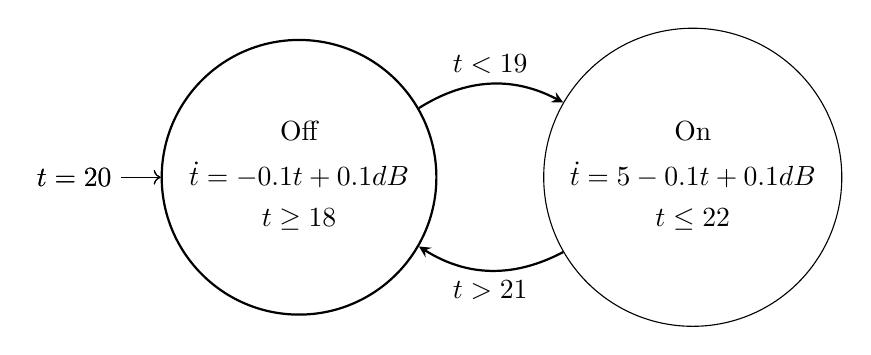
\begin{tikzpicture}
    \node (off) [state,
        initial,
        initial left,
        initial distance=.5cm,
        thick,
        initial text=$t\eq20$] {$\begin{gathered}\text{Off}\\\dot{t} = -0.1t + 0.1 dB\\t\geq18\end{gathered}$};
    \node (on) [state] at (5,0) {$\begin{gathered}\text{On}\\\dot{t} = 5-0.1t + 0.1 dB\\t\leq22\end{gathered}$};
    \path [-stealth, thick]
    (off) edge[bend left] node [above]{$t<19$}   (on)
    (on) edge[bend left] node [below]{$t>21$} (off);
\end{tikzpicture}
\caption{Thermostat hybrid automaton, adapted from Henzinger~\cite{henzinger00}}\label{fig:thermostat}
\end{center}
\end{figure}

This is a thermostat operating in a stochastic environment, displayed in the style of hybrid automata~\cite{henzinger00}. It has two states, on and off, which it can jump between when the jump conditions are met. The continuous evolution of the temperature is given by stochastic differential equations, which combine deterministic drift with a stochastic noise component. dB refers to the differential of the Brownian motion process. This modelling paradigm allows us to better represent systems that experience stochastic interference since we can model the noise directly. In our example, temperature may fluctuate randomly but it will tend to increase when the heating is on, and slowly decrease when it is turned off.

\section{Mathematical background}\label{sec:background}
In order to formally state and reason about these we will need notions from probability and measure theory. We base our development on the probability theory developed by H{\"o}lzl and Heller~\cite{holzl11, holzlphd}. They develop the theory of the basic probability theory objects, such as measure spaces, measurable functions, and the Lebesgue integral.

\subsection{Measure theory}
A measure is a set function that is positive and countably additive. Probability is a measure that assigns 1 to the entire space; this property is often not necessary in our proofs, so we often do our mathematics in the more general setting of measure theory.

For discrete spaces, we are able to assign a measure to every subset. However, when working with uncountably infinite spaces this is no longer possible, so we restrict the sets that can be assigned a measure. The measurable sets form a structure called a \(\sigma\)-algebra, which is closed under complements and countable union. A measure space is a triple \((\Omega, \mathcal{F}, \mu)\) such that \(\mathcal{F} \subseteq 2^\Omega\) is a sigma algebra on \(\Omega\) and \(\mu\) is a measure on \(\mathcal{F}\). A very common \(\sigma\)-algebra is the Borel \(\sigma\)-algebra \(\mathcal{B}\), which is the \(\sigma\)-algebra generated by the open sets of a topological space. It is the canonical measurable space for any topological space - in particular the real numbers with the interval topology. Unless otherwise specified, if we are working in a topological space we will be using the Borel sets as the measurable sets.

Measurable functions are those that preserve the structure of the measurable space: Let \((X, \mathcal{F})\) and \((Y, \mathcal{G})\) be two measurable spaces. \(f : X \to Y\) is \(\mathcal{F} - \mathcal{G}\) measurable if for any \(S \in \mathcal{G}\), \(\{x \mid f(x) \in S\} \in \mathcal{F}\). In the setting of probability theory, measurable functions are called random variables. Measurable functions induce a measure on their target space given a source measure. We call this the distribution of the function: \(\mathcal{D}_f(S) = \mu(\{x \mid f(x) \in S\})\).

The Lebesgue integral is defined for measurable functions, and generalises the Riemann integral by allowing us to integrate functions with respect to any measure. It satisfies many properties, among them monotone convergence: \[\int \lim_{n \to \infty} f_n d\mu = \lim_{n\to\infty}\int f_n d\mu\]

We state that a property P holds almost everywhere (a.e.) if \(\{x \mid \lnot P(x)\}\) is a subset of a measurable set with measure 0 (a null set).

A natural setting for iterated experiments is the product space. Given an index set I and a collection of measures \((\Omega_i, \mathcal{F}_i, \mu_i)\), the product measure \[\prod_{i\in I} (\Omega_i, \mathcal{F}_i, \mu_i)\] is generated by sets of the form \(\{A \mid \forall i \in I. A_i \in \mathcal{F}_i\}\). The variable \(X_J\) for \(J \subseteq I\) is the projection from the product space with index \(I\) to index \(J\) - this helps us characterise product spaces with infinite index sets by considering their finite-dimensional distributions.

Exclusive to probability measures is the notion of independence: two families of events X and Y are independent with respect to probability measure \(\mu\) if \(\forall x \in X, y \in Y. \mu(x)\mu(y) = \mu(xy)\). Further, random variables are independent if their preimages are independent of each other.

To illustrate these concepts, consider the probability space of coin tosses: let \[(\Omega, \mathcal{F}, \mu) = \left(\{H,T\}, 2^{\{H, T\}}, \lambda S.\frac{\#S}{2}\right)\]

We can verify that it is a probability space because our measure assigns 1 to the space \(\Omega\). We can define the random variable into the integers:
\begin{definition}\label{def:coin_toss}
 \[C(\omega) = \begin{cases}
    \,1 & \text {if } \omega = H \\
    -1  & \text{if } \omega = T\\
\end{cases}\]
\end{definition}

Random variables allow us to take the distribution of our sample space and embed it in a space of interest. We can for example now show that the expected value of \(C\) is 0. Moreover, consider the product space over the probability space defined above: \[\prod_{1,2} (\Omega, \mathcal{F}, \mu)\] We can define random variables \(C_i(\omega) = C(\omega_i)\), and show that \(C_1\) is independent from \(C_2\).

\section{Stochastic processes}\label{sec:process}
A stochastic process is an indexed family of random variables from some probability space \(\{X_t \mid t \in I\}\) for random variables \(X_t\) and index set I. In many instances I represents time; a common choice is the natural numbers or the interval \([0, \infty)\). We define stochastic processes in Isabelle using a locale:

\Snippet{stochastic_process}

\noindent A locale is a named set of fixed variables and assumptions\cite{haftmann09}. One can define lemmas within the locale, which take on the locale assumptions and fixed variables, and gain access to other lemmas in the locale. Our stochastic process locale extends \texttt{prob\_space}, another locale which fixes \texttt{M :: 'a measure} and assumes it is a probability space. To these assumptions we add three fixed variables: \(M'\) is the target measurable space of our process, \(I\) is the index set, and X is the process itself. We then assume that that \(X_i\) is a random variable for all \(i\) --- the notion of random variable is defined within \texttt{prob\_space} as a measurable function with source \(M\). We add the \texttt{[measurable]} theorem attribute to our assumption, which tags it as part of the named theorem set \texttt{measurable} and enables the use of the measurability tactic, which will use this fact to prove subgoals related to measurability of our process.

Locales also give us a predicate that characterises the locale assumption. We define the stochastic process type as a quadruple which contains the source and target measures for the process, the index set, and the process itself, and which satisfies the conditions of \texttt{stochastic\_process}:
\Snippet{stochastic_process_typedef}

This improves automation, as properties of stochastic processes hold automatically for objects of the stochastic process type, rather than having to encode this as part of the assumptions of a lemma.

Brownian motion is a stochastic process characterised by four conditions:

\begin{enumerate}
   \item \(W_0 = 0\).
   \item Independent increments.
   \item Normally distributed increments.
   \item Almost surely continuous paths.
\end{enumerate}

It is ideally suited as a starting point for modelling real-world noisy systems. Independent increments mean that the process is Markov, normally distributed increments are well-behaved and appropriate for many situations because of the central limit theorem, and a.s. continuous paths make the process suitable for modelling physical phenomena, which cannot have discontinuities. A key contribution of this paper is the Kolmogorov-Chentsov theorem, which supplies a continuous modification of some process.

We define the distributions of the process - given some \(J \subseteq I\), we define a product measure where the distribution at each index is given by the process:

\[X_J = \prod_{j \in J} \mathcal{D}(X_j)\] % TODO: Needs refinement

To illustrate this concept, let \(\{C_i \mid i \in \mathbb{N}\}\) be a family of independent random variables such that each \(C_i\) is equal in distribution to \(C\). To construct this family, we can use the stream measure as our sample space, and \(C_i\left(\omega\right) = C(\omega_i)\). These variables are independent because they are isomorphic to the coordinate projections of the product measure from the naturals, which are independent by definition. By the same argument they are random variables into the Borel sets.

We can now construct the one-dimensional simple random walk process: \[W_i(\omega) = \sum_{n=1}^iC_n(\omega)\]

In the discrete case, integration reduces to normalised summation and all functions are measurable, so we can prove that \[E[W_i] = 0\] for all \(i\) by a straightforward induction.
% TK Brownian motion is the scaling limit of a random walk

When we want to consider the distribution induced by the entire process we can use the Daniell-Kolmogorov theorem, which has been formalised in Isabelle~\cite{immler12} and states that for any stochastic process there exists a product measure that agrees with it on all finite-dimensional distributions. It is the starting point for our formalisation, but it is not sufficient to prove existence of Brownian motion because we need that the process satisfy additional conditions that are not guaranteed by the Daniell-Kolmogorov theorem.

We further define processes with independent and stationary increments. A process has independent increments if for all \(t_0,\dots,t_n\) with \(t_0 < t_1 < \dots < t_n\), all \((X_{t_i} - X_{t_{i-1}})_{i=1\dots n}\) are mutually independent. In Isabelle, we define increments as sorted lists: a suitable stochastic process has independent increments if for any sorted list of a least two indices drawn from index set I, every successive pair of variables are independent. This is formalised using  the "indep\_var" property, which is part of HOL-Probability.

In order to compare processes, we first introduce the concept of compatible processes, which share the same index set, target measure, and source sigma algebra. Any two compatible processes X and Y are modifications of each other if, for any given $t \in I$, $P[X_t = Y_t] = 1$ Equivalently, X is a modification of Y iff there exists a family of null sets $N_t$ such that $\{X_t \neq Y_t\} \subseteq N_t$ for all $t \in I$.

\begin{lemma}
Let X and Y be modifications of each other with index set I. Then \[(X^J) = (Y^J) \text{ in distribution}\qquad \text{ if } J \subseteq I\]
\end{lemma}
This follows from the fact that if two random variables are almost surely equal then their distributions are equal, and product measures are equal iff all their components are.

With modifications, it might still be the case that the set $\{\exists t. X_t \neq Y_t\}$ is not a null set, since an uncountable union of null sets is not necessarily null. Two processes X and Y are indistinguishable if the set $\{\exists t. X t \neq Y t\}$ is indeed a null set.

If two processes are indistinguishable then they are modifications of each other, since indistinguishability gives us a null set that fits the requirements of modification. In the other direction, we can show that modifications are indistinguishable on a countable index set: Assume that X and Y are modifications of each other. Then we can obtain a null set $N_t$ such that $\{X_t \neq Y_t\} \subseteq N_t$. By countable additivity, $\bigcup_t N_t$ is also a null set, proving our theorem.

We also show another condition for equivalence of modification and indistinguishability:

\begin{lemma}
Let X and Y be stochastic processes into a metric space \((S, d)\) which are modifications of each other, and that their index takes the form \([0,T]\). Assume that X and Y are almost surely continuous. Then X and Y are indistinguishable.
\end{lemma}

The proof of this theorem relies on obtaining a null set for a countable dense subset of the index space, and extending the null set to cover the whole space by continuity. We also rely on this technique later for the proof of the Kolmogorov-Chentsov theorem. For this use the dyadic rationals: numbers of the form \(\frac{k}{2^n}\) where \(k, n\in\mathbb{N}\). We present a novel definition for the sets of dyadic rationals with denominator \(2^n\) covering intervals of reals \([0,T]\) as follows:
 \[D_n(T) = \left\{\frac{k}{2^n} \mid k \in 0 \ldots\left\lfloor 2^nT \right\rfloor\right\}\]
With this, we define the dyadic rationals \(D(T)= \bigcup_n D_n(T)\). By showing that any real is a limit of a sequence of dyadic rationals, we can use the dyadics to bridge the gap between countable and uncountable sets.

\section{Transition kernels}\label{sec:kernel}
Transition kernels can be understood as generalisations of the transition functions of Markov chains. They can be used to characterise and construct Markov processes in a natural way, and we will use them to construct our Brownian motion process. In this section we develop the machinery required for defining stochastic processes using well-behaved families of kernels. This will involve defining the infinite product space generated by a family of kernels, building on the Daniell-Kolmogorov theorem, whose coordinate process will have the desired properties. In particular, we are concerned with Markov semigroups: consistent families of kernels where composing kernels is equivalent to adding their indices.

We define a transition kernel from measurable space \((\Omega, \mathcal{A})\) to \((\Omega', \mathcal{A}')\) as a function \(\kappa: \Omega \times \mathcal{A}' \to \mathbb{R}^+\) such that:
\begin{align*}
\forall A' \in \mathcal{A}'.\quad& \kappa(-, A') \text{ is } \mathcal{A} - \mathcal{B}\text{ measurable}\\
\forall \omega \in \Omega.\quad& \kappa(\omega, -) \text{ is a measure on } (\Omega', \mathcal{A}')
\end{align*}

If we assume we're in state \(\omega\), \(\kappa(\omega, A')\) is a function that gives us the probability of ending up in some state in \(A'\). Transition kernels provide a natural way of defining processes by characterising its increments. 
In Isabelle we define them as a locale:
\Snippet{transition_kernel}

A transition kernel \(\kappa : \Omega \to A'\) is stochastic iff \(\forall \omega \in \Omega. \kappa(\omega, -)\) is a probability measure, and likewise for finite kernels.

As an example of a stochastic kernel, consider the random walk process defined above. For countable state spaces, kernels are uniquely defined by their action on singleton sets. A single random walk step is defined by:

\[\kappa(n, \{m\}) = \frac{\delta_{n+1, m} + \delta_{n-1, m}}{2}\]

Where \[\delta_{x,y} = \begin{cases}
    1 &\text{if } x = y\\
    0 &\text{otherwise}
\end{cases}\] is the Kronecker delta. When starting in state n, the transition kernel gives probability \(\frac{1}{2}\) to states \(n+1\) and \(n-1\), and 0 otherwise. The kernel has to be countably additive, so we can define its action on an arbitrary set as the sum of its action on its members. For fixed n, the above kernel defines a probability measure. All functions on the discrete measurable space are measurable, so this is a stochastic kernel.

Other useful kernels include the measure kernel \(\kappa_\mu(\omega, A) = \mu(A)\) which lifts a measure \(\mu\) to the kernel setting, ignoring its first argument, and the indicator kernel \(\delta(\omega, A) = \mathbb{1}_A(\omega)\), which is analogous to a skip operation in programming -- it represents the identity transition.

In order to compose kernels together we need to integrate with respect to the kernel measure. We show that this integral is measurable, which is essential if we are composing several integrals, or defining a kernel in terms of the integral of another kernel.
\begin{lemma}
    Define \[I_f(\omega_1) = \int f(\omega_1, \omega_2) \kappa(\omega_1, d\omega_2)\]
    Let f be an \((\Omega_1 \times \Omega_2 - \mathcal{B})\) measurable function. Let \(\kappa\) be a finite kernel on \(\Omega_1 - \Omega_2\). Then \(I_f\) is a Borel measurable function.
\end{lemma}

The proof for this lemma follows a standard approximation approach for Borel measurable functions:
 We first show that \(\mathbb{1}_S\) is measurable if \(S\) is a measurable set by proving that the set \(\{S \mid I_{\mathbb{1}_S} \text{ is measurable}\}\) forms a Dynkin system with rectangles \(X \times Y\) as generators. Next, we can show that any simple function is measurable, since they are simply finite sums of indicator functions multiplied by constants. Finally, this allows us to approximate any Borel measurable function using monotone convergence.

\subsection{Kernel Product}
The binary kernel product combines two kernels to operate on a product space. Let \(\kappa_1\) be an \(\Omega_1 - \Omega_2\) kernel, and \(\kappa_2\) be a \(\Omega_1 \times \Omega_2 - \Omega_3\) kernel. Then the kernel product \(\otimes_K\) is a kernel \(\Omega_1 - \Omega_2 \times \Omega_3\) such that
\[(\kappa_1 \otimes_K \kappa_2)(\omega_0, A) = \int\left(\int \mathbb{1}_A(\omega_1, \omega_2)\kappa_2((\omega_0, \omega_1)d\omega_2)\right)\kappa_1(\omega_0, d\omega_1)\]

We also define \(\otimes_P\) as the kernel product of \(\kappa_1: \Omega_1 - \Omega_2\) and \(\kappa_2: \Omega_2 - \Omega_3\) by understanding \(\kappa_2\) as a kernel that ignores the elements of \(\Omega_1\). This operation has more reasonable types which makes it more compositional, and therefore more useful in defining stochastic processes.

We show that our definitions form a transition kernel if the kernels are finite. For this, we need to prove that the inside of the integral is measurable, which requires an additional proof. The arguments for these are quite standard - approximation using Dynkin systems. If both kernels are finite then the product is \(\sigma\)-finite, and if they are stochastic or substochastic then the product is too.

Our objective is to define the finite product kernel analogously to the following recursion:
\[\bigotimes_{i=1}^{k+1} \kappa_i = (\kappa_1 \otimes \kappa_2 \otimes \dots \otimes \kappa_{k}) \otimes \kappa_{k+1}\]

This would require dependent types, and it would not be compatible with the existing product measure. Instead, we define it using the product measure \texttt{PiM} as our target.

Let \texttt{n} be a natural number, \texttt{I} an injection from \([0,n]\) into an index set, and \texttt{K} a family of kernels with index set \(\texttt{I}([0,n])\). Then \[\bigotimes_{k=0}^n K_{I_k}\] is a kernel \(\Omega - \Omega^I\). We define this by recursion: the base case lifts kernel K 0 to operate on the dependent function space, and the recursive case defines the product kernel as an integral with respect to K (Suc n), analogously to our binary product construction. We show that this kernel is well-formed by induction on n, reusing proofs for the partial binary product in the inductive case.

We use the product kernel to define a construction using convolution:
\begin{lemma}\label{lemma:convolution}
Given a family of independent variables \(X_i\) and index I, define the kernels \[\kappa_i(\omega, A') = (\delta_\omega \star \mathcal{D}(X_i))(A')\] The product kernel of \(\kappa_i\) at state 0 is equal to the distribution of \(X_i\):
\[\left(\bigotimes_{k=0}^n \kappa_{I_k}\right) 0 = \prod_{t\in I([0,n])}\mathcal{D}(X_t)\]
\end{lemma}

We now define a way of obtaining a measure from a kernel. Let \((\Omega, \mathcal{F}, \mu)\) be a measure space, and let \(\kappa: \mathcal{F} - \mathcal{G}\) be a finite kernel. Then
\[\mu \otimes_S \kappa = \kappa_\mu \otimes_P \kappa\]
defines the semidirect product. We prove that integrals over the semidirect product can be split into two integrals:

\[\int f(\omega) (\mu \otimes_S \kappa)(d \omega) = \int \left(\int f(\omega_1, \omega_2) \kappa(\omega_1, d\omega_2)\right) \mu(d\omega_1)\]

Finally, we define kernel composition. Let \(\kappa_1\) be a finite \((\Omega_0, \mathcal{A}_0) - (\Omega_1, \mathcal{A}_1)\) transition kernel, and let \(\kappa_2\) be a \((\Omega_1, \mathcal{A}_1) - (\Omega_2, \mathcal{A}_2)\) transition kernel. We can now define kernel composition by \[\kappa_1 \circ \kappa_2(\omega_0, A_2) = \int_{\Omega_1} \kappa_2(\omega_1, A_2) \kappa_1(\omega_0, d\omega_1) \]

\subsection{Markov semigroups}
Let \(\kappa_{i,j} :I \to I \to \Omega \to \mathcal{A}\) be a family of stochastic kernels on \((\Omega, \mathcal{A})\), where I is an ordered set. \(\kappa\) is a consistent family if:
\[\kappa_{i,j} \circ \kappa_{j,k} = \kappa_{i,k} \qquad \text{ for } i,j,k \in I\]

Using the finite kernel product, we show that consistent families of kernels form a projective family, and therefore we can construct an infinite product kernel using them.

\begin{lemma}
For any consistent family of stochastic kernels \(E - E\) with index set \(I \subseteq [0, \infty)\) containing 0, we show there is a kernel \(E - E^I\) such that, for all sets \(J \subseteq I = \{j_1, j_2, \dots, j_n\}\) where \(j_1 < j_2 < \dots < j_n\): 
    \[\kappa(x, -) \circ X_J^{-1} = \left(\delta_x \otimes_S \bigotimes_{k=0}^{n-1} \kappa_{j_k, j_{k+1}}\right)\]
\end{lemma}

Now consider the stochastic family of kernels \(\kappa_i : I \to \Omega\to \mathcal{A}\) on \((\Omega, \mathcal{A})\). \(\kappa_i\) is a Markov semigroup if
\begin{align*}
    \kappa_0(\omega, -) &= \delta_\omega\\
    \kappa_s \circ \kappa_t &= \kappa_{s+t}
\end{align*}

Any Markov semigroup \(\kappa\) is a consistent family defined by \(\kappa_{s,t} = \kappa_{t-s}\). The infinite product kernel defined by a Markov semigroup is particularly well-behaved, and defines a process with stationary, independent increments.

Using this, we can construct a stochastic process with independent, stationary increments for any family of distributions that satisfy the property \(\nu_{t+s} = \nu_t \star \nu_s\) using lemma \ref{lemma:convolution}.

\section{Kolmogorov-Chentsov}\label{sec:modification}
The Kolmogorov-Chentsov theorem allows us to construct continuous modifications of processes which satisfy some conditions on their expectations. We first present some preliminary concepts needed for the statement and proof of the theorem:

\subsection{H{\"o}lder continuity}
Let \((E, d)\) and \((E', d')\) be two metric spaces. A function \(\varphi: E \to E'\) is locally H{\"o}lder continuous of order \(\gamma\) (H{\"o}lder-\(\gamma\)-continuous) for \(0 < \gamma \le 1\) on set \(D\) if for all \(t \in D\) there is an \(\varepsilon > 0\) and a \(C \ge 0\) such that
\[\forall r, s \in B_t(\varepsilon)\cap D. d(\varphi(r), \varphi(s)) \le  C d'(r,s)^\gamma\]

Where \(B_t\) is the open ball centred around t. \(\varphi\) is \(\gamma\)-(globally) H{\"o}lder continuous on D if we don't restrict r and s to be in some neighborhood of t - that is, if there exists some \(C \ge 0\) s.t.
\[\forall r, s \in D. d(\varphi(r), \varphi(s)) \ge C d'(r,s)^\gamma\]

Clearly, if \(\varphi\) is H{\"o}lder-\(\gamma\)-continuous on D it is also locally H{\"o}lder-\(\gamma\)-continuous on D. The other direction holds if D is compact - we prove this by constructing the constant C required by global continuity using the constants given by local continuity on the finite open cover of D.

We show the relationships between H{\"o}lder continuity and other forms of continuity: global 1-H{\"o}lder continuity is Lipschitz continuity and local 1-H{\"o}lder continuity is local Lipschitz; global \(\gamma\)-H{\"o}lder implies uniform continuity and both global and local imply regular continuity.

\subsection{Kolmogorov-Chentsov theorem}
We first prove a generalised version of Markov's inequality:

\begin{lemma}
Let \((\Omega, \mathcal{A},\mu)\) be a measure space, Let X be a real-valued measurable function on \(\mathcal{A}\). Let \(f: \mathbb{R} \to [0, \infty)\) be monotonically increasing on the set \((0, \infty) \cup ran(X)\). Then, for any \(\varepsilon > 0\) where \(f(\varepsilon) > 0\):
\[\mu [X(p) \ge \varepsilon] \le \frac{\int_\Omega f (X(x)) \mu(dx))}{f(\varepsilon)}\]
\end{lemma}

With this we can prove our main result:

 \begin{theorem}
Let X be a stochastic process that takes values in a polish space, with index set \([0..\infty)\). Assume there exist numbers \(\alpha, \beta, C > 0\) such that X satisfies the following property: 
\[E[d(X_t, X_s)^\alpha] \leq C |t - s|^{1+\beta}, s,t \in \mathbb{R}^+\]

Then there is a modification Y of X such that for any \(\gamma \in (0..\beta/\alpha)\), Y H{\"o}lder-continuous paths of order \(\gamma\).
 \end{theorem}
\begin{proof}
Because distance is measurable, we have that \(d(X_s, X_t)\) is a real-valued random variable. We can then apply Markov's inequality above, with \(f(x) = x^a\), to obtain the following:
\[P[d(X_s, X_t) \le \varepsilon] \le \frac{E[d(X_t, X_s)]^\alpha}{\varepsilon^\alpha}\]

By assumption, it then follows that
\[P[d(X_s, X_t) \le \varepsilon] \le \frac{C|t-s|^{1+\beta}}{\varepsilon^\alpha}\]

It then follows that \(X_s\) converges in probability to \(X_t\). We will construct our modification as a limit of the process as \(s \to t\), and because \(X_s\) converges in probability this will allow us to show that the limit is equal to \(X_t\) with probability 1, and hence a modification.

Fix \(T > 0\). We construct a H{\"o}lder-continuous modification of X restricted to \([0, T]\), and then show that we can extend these modifications to the interval \([0, \infty)\).

For this, we will define a null set which characterises the paths that are not H{\"o}lder-continuous.

Define
\[A_n = \{\text{Max } \{d(X_{2^{-n}(k-1)}, X_{2^{-n}k}) \mid k \in 1..\left\lfloor 2^nT\right\rfloor\} \ge 2 ^ {-\gamma n}\}\]
\[B_n = \bigcup_m A_{m+n}\]
\[N = \bigcap_n B_n\]

\(P(B_n)\) tends to 0 as \(n \to \infty\), which allows us to show that N is a null set. We then fix \(\omega \in \Omega - N\) and show that \(\lambda t. X_t \omega\) is H{\"o}lder continuous on the dyadic rationals. H{\"o}lder continuity implies uniform continuity, and therefore \(\lim_{s\in D \to t} X_s(\omega)\) is defined. Define \[\tilde{X}_t = \text{if } t \in D \text{ then } X_t(\omega) \text{ else } \lim_{s\in D \to t} X_s(\omega)\] We show that our constructed process is H{\"o}lder continuous, and equal to the original one almost everywhere by convergence in probability.

We have now proven that for any T, there is a H{\"o}lder-\(\gamma\)-continuous modification of X on \([0,T]\). Any two modifications on \([0, S]\) and \([0,T]\) are indistinguishable on \([0, \text{min}(S, T)]\) because they are continuous. Therefore, for \(S, T > 0\) we have a null set \(N_{S,T}\) such that \({X^T \neq X^S} \subseteq N_{S,T}\). Then, \(N' = \bigcup_{S, T \in \mathbb{N}} N_{S, T}\) is a null set by countable subadditivity. Define \(\tilde{X} = X\) on all \(\omega \in \Omega - N'\). Then, \(\tilde{X}\) restricted to T is equal to \(X^T\), and hence H{\"older} continuous on \(\Omega - N'\). Furthermore, it is a modification of X, completing our proof.
\end{proof}

\subsection{Brownian motion}\label{sec:brownian-motion}
We define Brownian motion using a locale:
\Snippet{brownian_motion}

Any process that satisfies these conditions is Brownian motion by definition. We can now construct a process that satisfies these using the theory that we have developed. Define the family of Brownian motion kernels by:

\[\kappa_t(\omega, A') = (\delta_\omega \star \mathcal{N}_{0, t})(A')\]

We show that this defines a Markov semigroup, and we can therefore use it to construct an infinite-dimensional product space. The coordinate process from this product space have the requisite distributions, and we prove that this process satisfies the requirements of the Kolmogorov-Chentsov theorem for all \(\gamma < \frac{1}{2}\), which yields a continuous modification of our process. We have shown the existence of the Brownian motion process.

% Formalise a process other than Brownian motion to display the generality
\section{Conclusion}\label{sec:conclusion}
We have developed a theory of stochastic processes in Isabelle/HOL, based on the existing probability theory library. We formalised stochastic processes and stochastic kernels, defined a way of constructing processes with kernels, and proved the Kolmogorov-Chentsov theorem for producing continuous modifications of well-behaved processes. We applied this theory in order to construct the Brownian motion process.

We found that on a number of occasions, the textbook proofs omitted a significant amount of detail, at times skipping proof obligations entirely. This was most common with measurability proofs, which can be quite tedious but were often dismissed by the author. Indeed, most of the work of formalising pen-and-paper mathematics lies in making the implicit explicit, and filling in the gaps between the broad strokes of the proofs.

In particular, one of the major deviations from the textbook was the development of the theory of dyadic intervals. In the proof of Kolmogorov-Chentsov, the author assumes ``without loss of generality'' that T=1, implicitly arguing that the reasoning for any other value of T would be identical. This kind of reasoning cannot be carried out ad hoc in a proof assistant, and we therefore had to develop a theory that allowed us to deal with arbitrary values of T in the proof, leading us to dyadic intervals.

At times, we also had to make concessions for the type system. The finite kernel product was defined in the textbook as a recursion using the binary product. This would need dependent types to work in Isabelle, so we again had to make this construction explicit. Other such occasions included having to restrict the types of measures to be homogeneous when they could in theory each have a different type, although we doubt this will have any impact in practice. The advantage of using simple types is the wealth of automation facilities available; much of the low-level reasoning can be deferred to automated theorem provers via Sledgehammer, making the development simpler.

Our development consists of approximately 5000 lines of proofs, formalising about 20 pages of the textbook.

In summary, we had to make concessions and interpret the text in order to produce our theory, but our proofs generally followed the same steps as the textbook. We have developed a method for constructing stochastic processes with stationary, independent increments which are continuous almost everywhere, and we then applied this method to construct Brownian motion. This is an important step towards developing a theory of stochastic differential equations in Isabelle/HOL, which will enable the deductive verification of stochastic hybrid systems.

%Outline future work. It's worth stating that you'll build a verification tool based on [1]. What are some research questions that you'd like to address with such a tool? Considering referring back to your stochastic thermostat.
 We plan to build on this work by developing a practical verification tool for SHS based on the hybrid systems verification tool by Foster et al.\cite{foster21}. Our objective is to be able to reason about safety and liveness properties of SHS, using a formalised mathematical background that gives us confidence in our foundations.

\printbibliography
\end{document}
